% Copyright 2007 by Till Tantau
%
% This file may be distributed and/or modified
%
% 1. under the LaTeX Project Public License and/or
% 2. under the GNU Public License.
%
% See the file doc/licenses/LICENSE for more details.



\documentclass{beamer}

%
% DO NOT USE THIS FILE AS A TEMPLATE FOR YOUR OWN TALKS¡!!
%
% Use a file in the directory solutions instead.
% They are much better suited.
%


% Setup appearance:

\usetheme{Darmstadt}
\usefonttheme[onlylarge]{structurebold}
\setbeamerfont*{frametitle}{size=\normalsize,series=\bfseries}
\setbeamertemplate{navigation symbols}{}


% Standard packages
\usepackage{url}
\usepackage{hyperref} 
\hypersetup{
    %colorlinks=true,
    %linkcolor= true,
    %filecolor= black,      
    urlcolor=blue,
}
\usepackage[english]{babel}
\usepackage[latin1]{inputenc}
\usepackage{times}
\usepackage[T1]{fontenc}
%\usepackage[longnamesfirst, authoryear]{natbib}
\usepackage{natbib}
\bibliographystyle{apalike}
\renewcommand\bibfont{\scriptsize}
%\usepackage[font=scriptsize,labelfont=bf]{caption}
% Setup TikZ
\usepackage{amsmath}
\usepackage{gensymb}
\usepackage{multimedia}
\usepackage{media9}
\usepackage{caption}
\usepackage[font=scriptsize, skip = 0pt]{caption}
\usepackage{subcaption}
\usepackage{tikz}
\usetikzlibrary{positioning}
\usetikzlibrary{arrows}
\tikzstyle{block}=[draw opacity=0.7,line width=1.4cm]
\beamertemplatetransparentcovereddynamic


% Author, Title, etc.

\title[] 
{Using Eclipse to Probe Physical Conditions Along the Jets in the X-Ray Binary SS 433%
}

\author[Liu]
{
  \textbf{Xinyi~Liu}\inst{1}
}

\institute[Wheaton College]
{
  \inst{1}%
 Wheaton College, MA
}

\date[\today]



%The main document

\begin{document}
\begin{frame}
  \titlepage
 Physics and Astronomy Department\\
 Thesis Defense \\
 May 9, 2018
  
\end{frame}

\begin{frame}{Outline}
  \tableofcontents
\end{frame}


\section{Introduction}

    
\subsection{SS 433 system}
% \begin{frame}{An X-ray Binary system}
% \begin{figure}
% \centering
% \begin{subfigure}[t]{.5\textwidth}
%   \centering
%   \includemedia[scale = 0.035\linewidth , activate=pageopen, passcontext, transparent, addresource=ss433binary.mp4, flashvars={source=ss433binary.mp4}
% ]{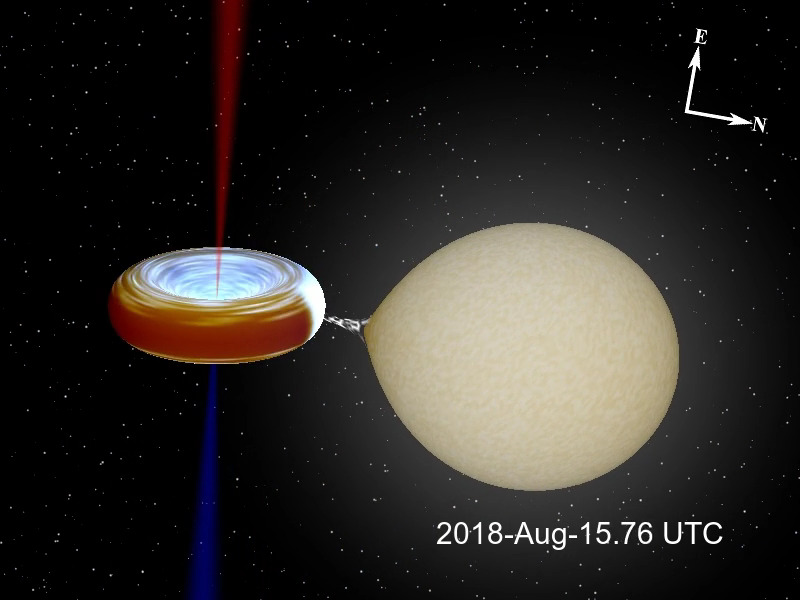
\includegraphics[width=0.17\linewidth]{binary1.jpg}}{VPlayer.swf}
%   %\movie{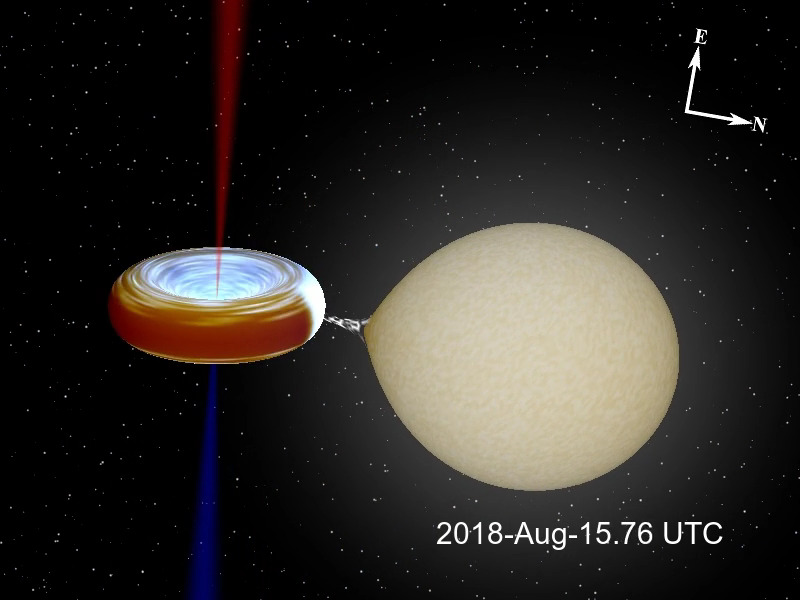
\includegraphics[scale = 0.17]{binary1.jpg}}{ss433_chandra_mjd.mp4}
%   \caption{The orbital motion of \href{http://dmaitra.webspace.wheatoncollege.edu/ss433_chandra_mjd.mp4}{binary system}}
%   \label{binary}
% \end{subfigure}%
% \begin{subfigure}[t]{.5\textwidth}
%   \centering
%   \includemedia[scale = 0.035\linewidth , activate=pageopen, passcontext, transparent, addresource=onlyjet.mp4, flashvars={source=onlyjet.mp4}
% ]{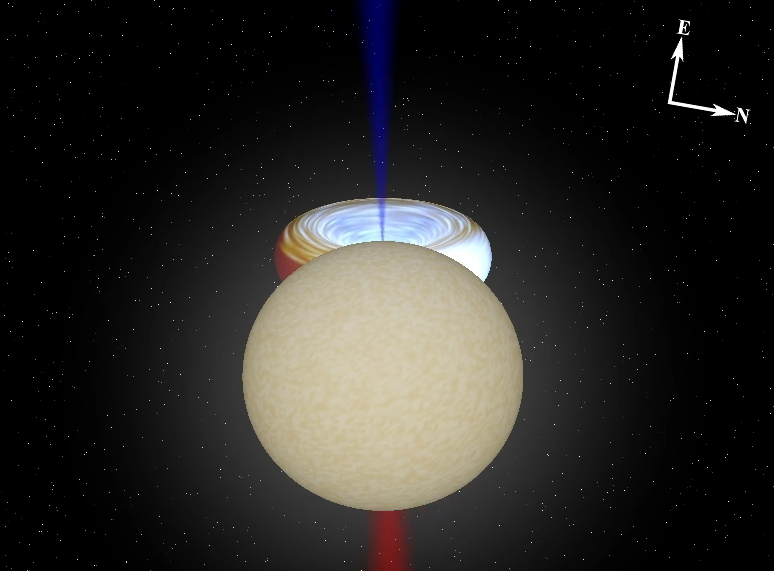
\includegraphics[width=0.17\linewidth]{jet.png}}{VPlayer.swf}
%   %\movie{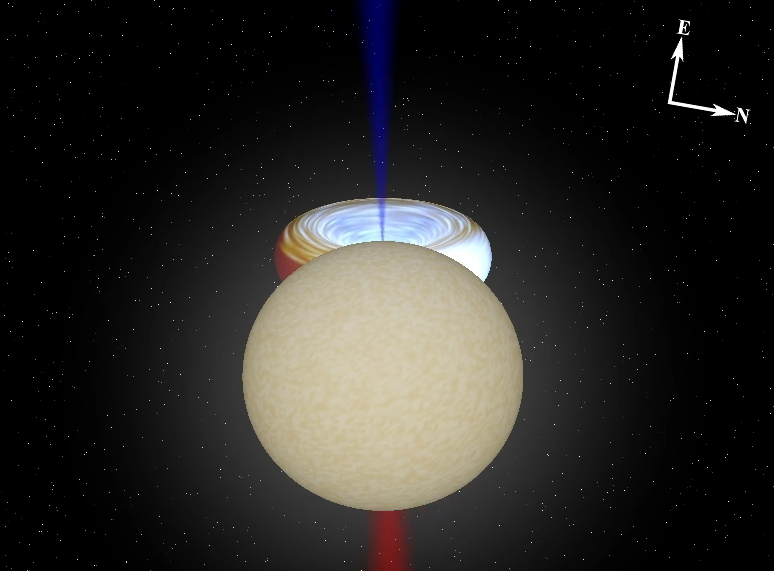
\includegraphics[scale = 0.18]{jet.png}}{only_jet_precession.mp4}
%   \caption{\href{http://dmaitra.webspace.wheatoncollege.edu/only_jet_precession.mp4}{Jet precession}}
%   \label{jet}
% \end{subfigure}
% \label{video}
% \end{figure}
    
% \end{frame} 

\begin{frame}{SS 433}
       \begin{columns}
          \column{0.45\linewidth}
          \begin{itemize}
             \item X-ray binary system
             \item Distance: 17.9 $\times 10^3$ light years
             \item Surrounded by W50 nebula
          \end{itemize}
         \column{0.5\linewidth}
          \begin{figure}
                \centering
                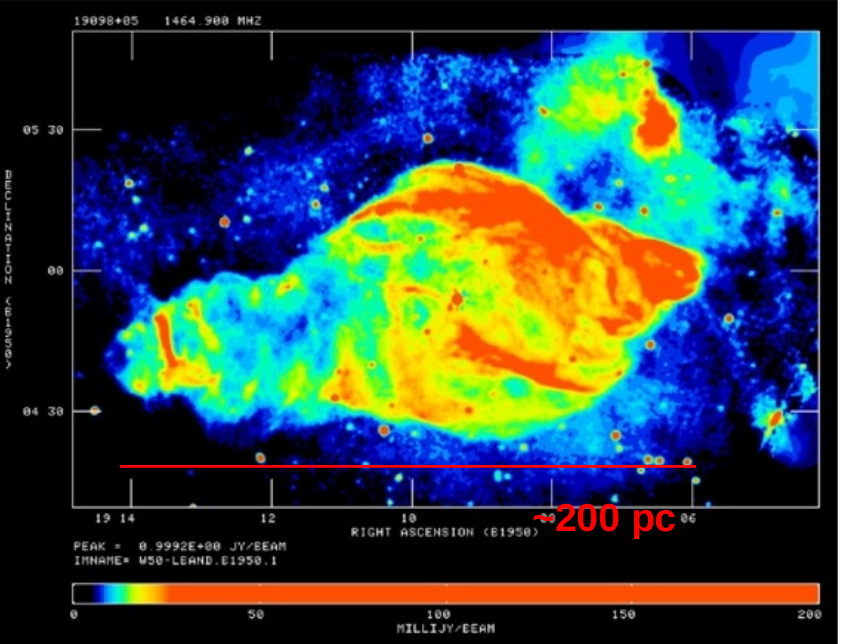
\includegraphics[scale = 0.2]{w50.png}
                \caption{W50 nebula, a supernova remnant.}
                \label{hess}               
                \end{figure}
          \end{columns} 
\end{frame}



\begin{frame}{An X-ray Binary system}
\begin{figure}
  \centering
  \includemedia[scale = 0.035\linewidth, activate=pageopen, passcontext, transparent, addresource=only_orbital_motion.mp4, flashvars={source=only_orbital_motion.mp4}
]{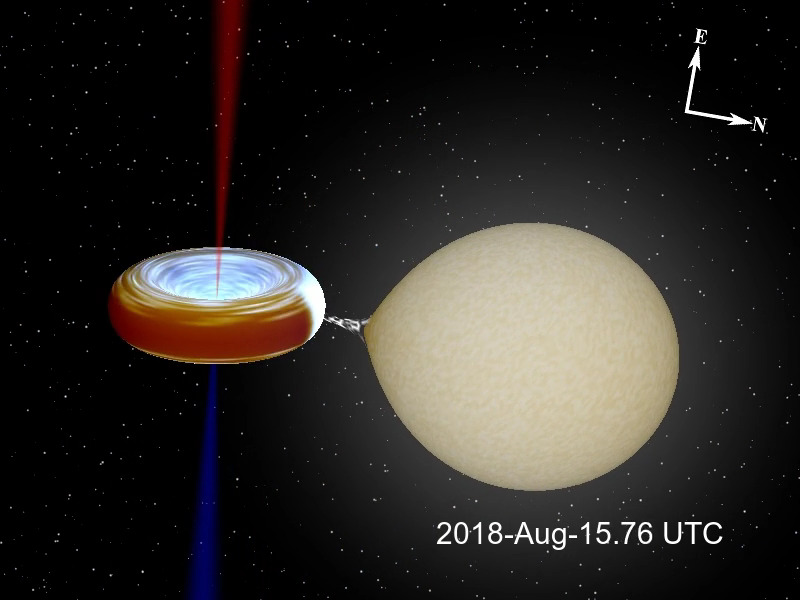
\includegraphics[width=0.07\linewidth]{binary1.jpg}}{VPlayer9.swf}
  %\movie{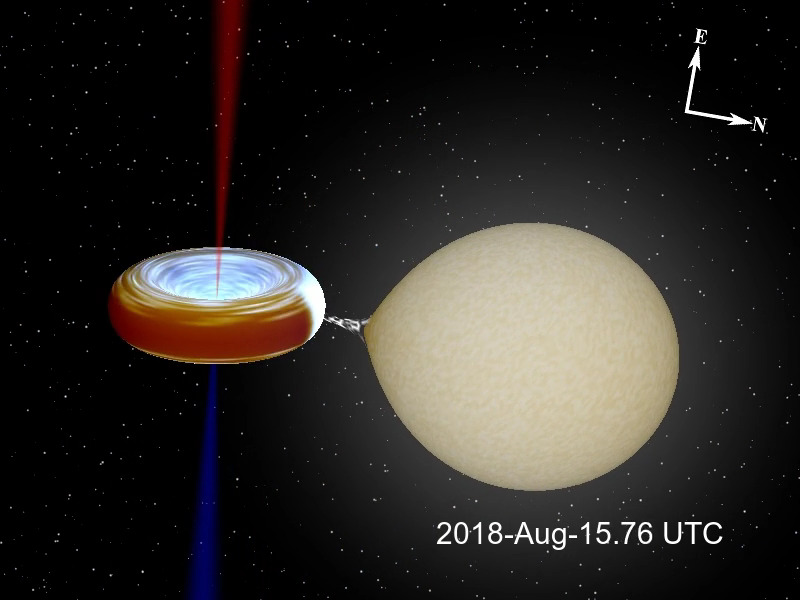
\includegraphics[scale = 0.17]{binary1.jpg}}{ss433_chandra_mjd.mp4}
  \caption{The orbital motion of \href{http://dmaitra.webspace.wheatoncollege.edu/only_orbital_motion.mp4}{a binary system}}
  \label{binary}
\end{figure}
\end{frame}




\begin{frame}{Jet Precession}
\begin{figure}
  \centering
  \includemedia[scale = 0.035\linewidth, activate=pageopen, passcontext, transparent, addresource=onlyjet.mp4, flashvars={source=onlyjet.mp4}
]{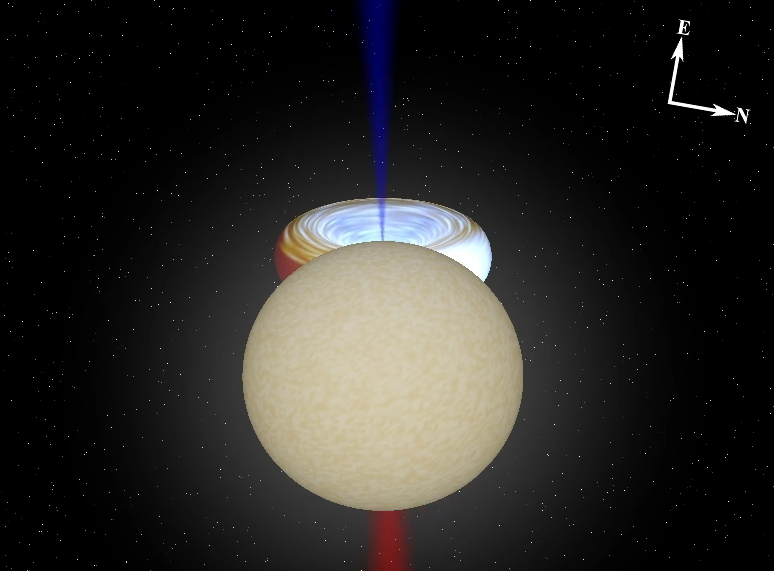
\includegraphics[width=0.07\linewidth]{jet.png}}{VPlayer9.swf}
  %\movie{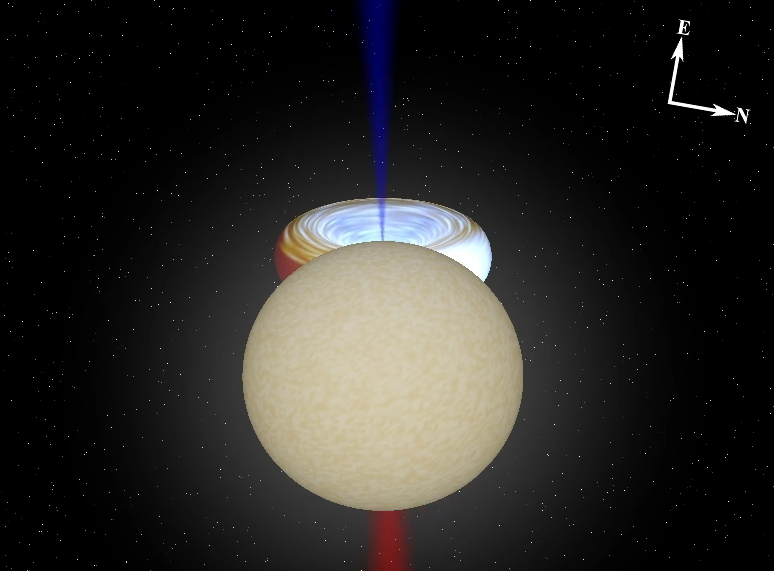
\includegraphics[scale = 0.18]{jet.png}}{only_jet_precession.mp4}
  \caption{\href{http://dmaitra.webspace.wheatoncollege.edu/only_jet_precession.mp4}{Jet precession}}
  \label{jet}
\end{figure}
\end{frame} 


%-----------------------------------------------
%-----------Motivation--------------------------
\subsection{Motivations}
\begin{frame}{Motivations}
    Fundamental questions in high-energy astrophysics
    \begin{itemize}
        \item Jet's launching mechanism
        \item The evolution of the physical conditions along the jet
        \end{itemize}
\end{frame}

\subsection{Some Physical Principles}
%---------------------------------------------
%--------emission lines--------------------
\scriptsize
\begin{frame}{Emission Lines}
       \begin{columns}
          \column{0.3\linewidth}
            \begin{figure}
                \centering
                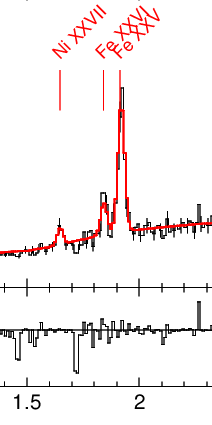
\includegraphics[scale = 0.3]{emission_lines.png}
                \caption{Some emission lines in the 1.5 - 2 \AA\ range.}
                \label{emission_lines}
            \end{figure}

          \column{0.6\linewidth}
          \begin{itemize}
              \item Hydrogen-like atom
          \end{itemize}
          \pause
          \begin{align*}
              |\dfrac{1}{4\pi \epsilon_0}\dfrac{-e(Ze)}{r^2}| &= \dfrac{m_ev^2}{r}\\
              \pause
              r &= \dfrac{4\pi\hbar\epsilon_0}{m_{e}Ze^2}n^2\\
              \pause
              E_n &= T + V = \dfrac{1}{2}mv^2 - \dfrac{Ze^2}{4\pi \epsilon_0 r} = \dfrac{Ze^2}{4\pi \epsilon_0 r}\\
              \pause
              E_n &= -\dfrac{me^4}{(4\pi\epsilon_0)^2\hbar^2}\dfrac{Z^2}{n^2} = -13.6 eV\ \dfrac{Z^2}{n^2}
          \end{align*}
          \pause
          E.g. Fe {\sc xxvi}, n = 2 $\rightarrow$ n = 1, where Z = 26
          \pause
          \begin{align*}
              E_{2\rightarrow1} = -13.6 eV [(\dfrac{26}{2})^2 -(\dfrac{26}{1})^2] &= 6.895keV \\
                                \lambda_{rest} &= 1.79 \textsc{\AA}
          \end{align*}
          \end{columns} 
\end{frame}


\begin{frame}{Relativistic Doppler Shift}
       \begin{columns}
          \column{0.4\linewidth}
            \begin{figure}
                \centering
                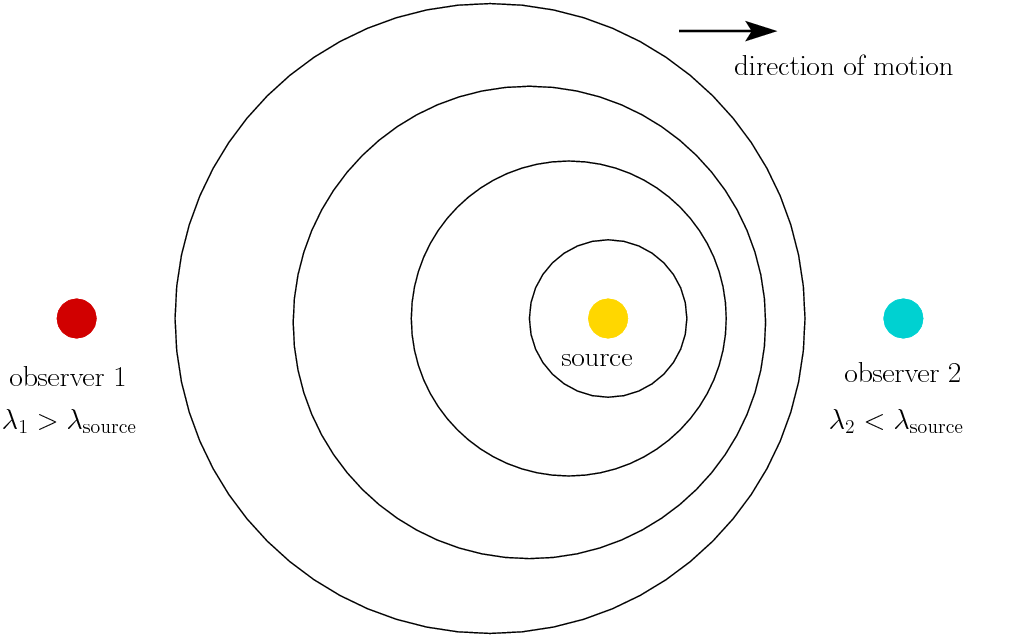
\includegraphics[scale = 0.14]{doppler.png}
                \caption{The Doppler effect occurs when the source and observer are traveling at different speeds relative to each other. }
                \label{emission_lines}
            \end{figure}
          \column{0.4\linewidth}
          \begin{itemize}
              \item $v \ll c$
          \end{itemize}
          \begin{align*}
              \lambda &= \lambda_0(1+\dfrac{v\mathrm{cos}\theta}{c})
          \end{align*}
          
          \pause 
          
          \begin{itemize}
              \item $v$ close to $c$
          \end{itemize}
          \begin{align*}
              \lambda = \dfrac{\lambda_0(1+\dfrac{v\mathrm{cos}\theta}{c})}{\sqrt{1-\dfrac{v^2}{c^2}}}
          \end{align*}
          \end{columns} 
\end{frame}


\begin{frame}{Transverse Doppler Shift ($\theta = 90$\textdegree)}
       \begin{columns}
          \column{0.45\linewidth}
            \begin{figure}
                \centering
                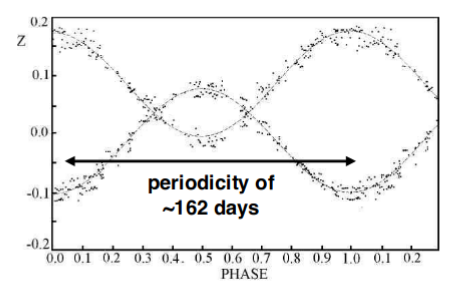
\includegraphics[scale = 0.4]{movingline.png}
                \caption{The periodic redshifts of both jets (GRAVITY et al., 2017)}
                \label{emission_lines}
           \end{figure}
           
          \column{0.4\linewidth}
          \begin{itemize}
              \item When $\mathrm{\theta}$ = 90\textdegree
          \end{itemize}
          \begin{align*}
              \lambda &= \dfrac{\lambda_0(1+\dfrac{v\mathrm{cos}(90\degree)}{c})}{\sqrt{1-\dfrac{v^2}{c^2}}}\\
              \pause
              \lambda &= \dfrac{\lambda_0}{\sqrt{1-\dfrac{v^2}{c^2}}}
          \end{align*}
          \pause
          \begin{itemize}
              \item Redshift
          \end{itemize}
          \begin{align*}
              z = \dfrac{\lambda- \lambda_{0}}{\lambda_{0}}
          \end{align*}
          \end{columns} 
\end{frame}










\section{Observation}
\subsection{Chandra Telescope}
\begin{frame}{Chandra Overview}
\begin{figure}
    \centering
    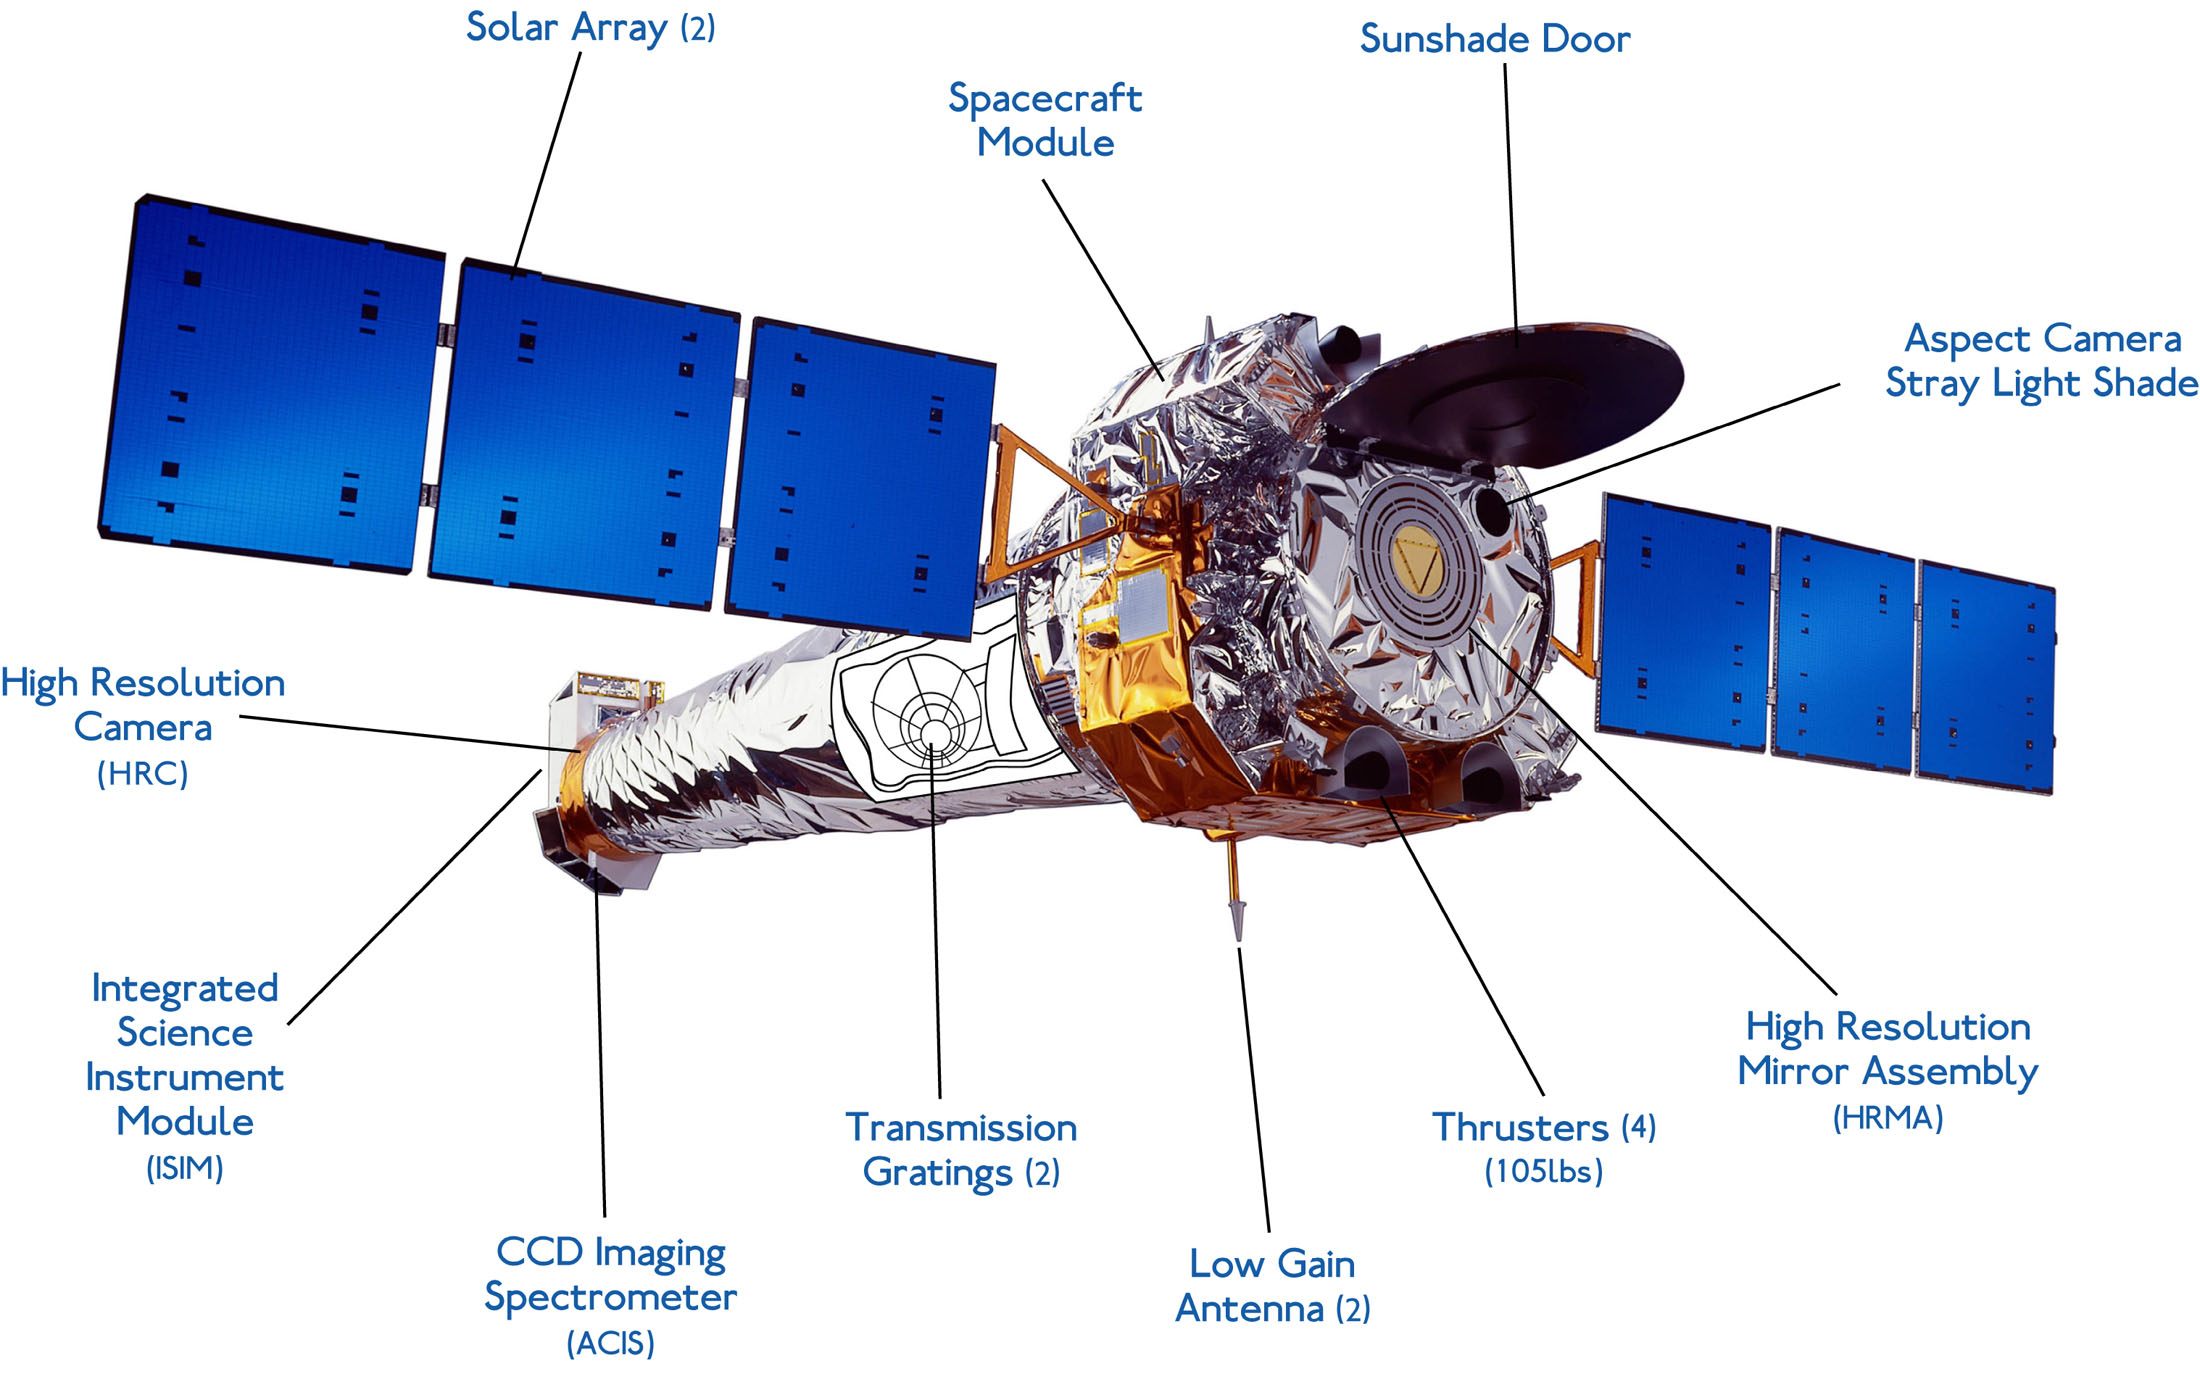
\includegraphics[scale = 0.4]{chandra_full.jpg}
    \caption{The Chandra Telescope with main components labeled \citep{Harbaugh2017}.}
    \label{chandra}
\end{figure}

    
\end{frame}

\normalsize
\begin{frame}{The Components of the Chandra}
\begin{figure}
    \centering
    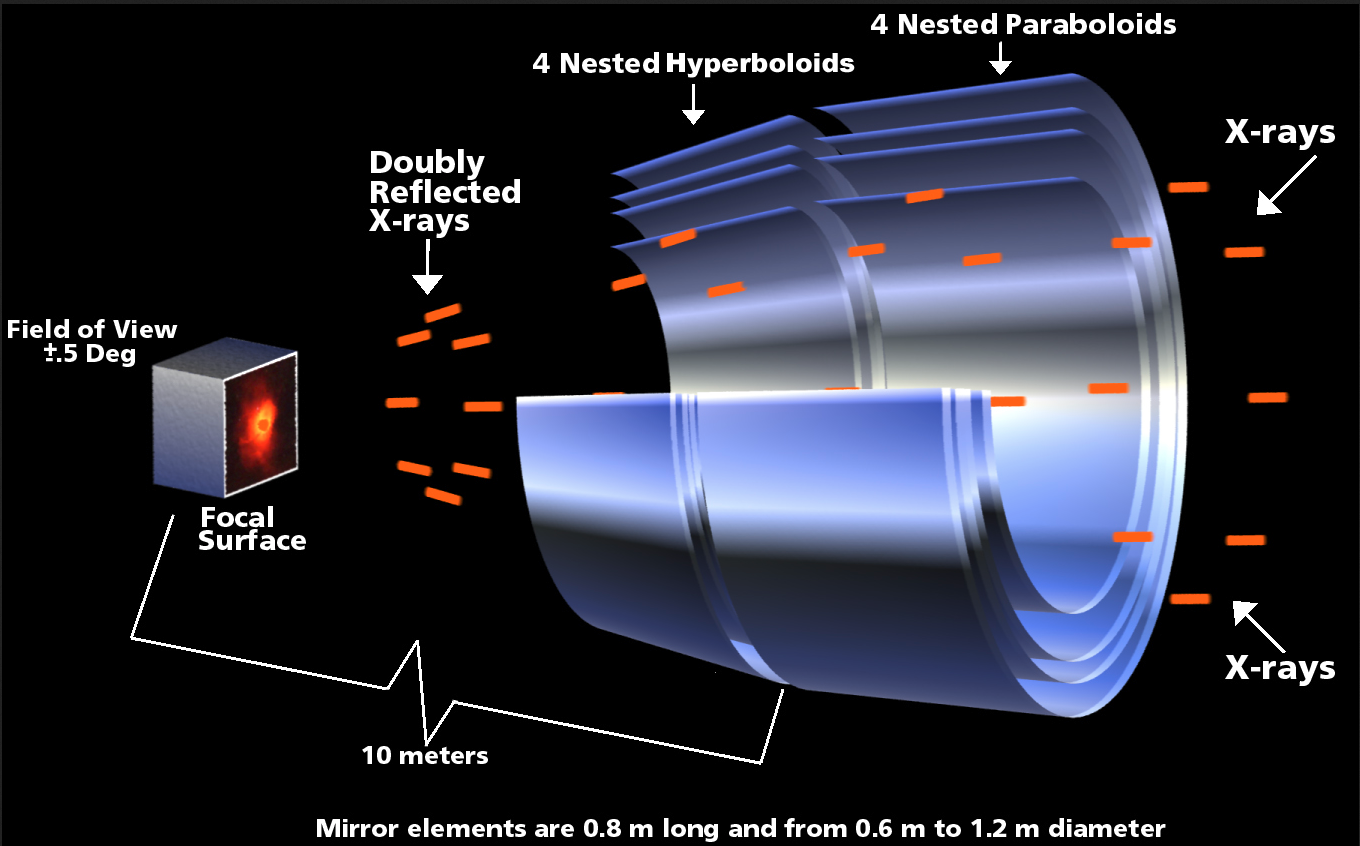
\includegraphics[scale = 0.2]{paraboloid_hyperboloid_mirror.png}
    \label{mirror}
\end{figure}
\end{frame}

\begin{frame}{High Energy Grating and Medium Energy Grating}
       \begin{columns}
          \column{0.45\linewidth}
            \begin{figure}
                \centering
                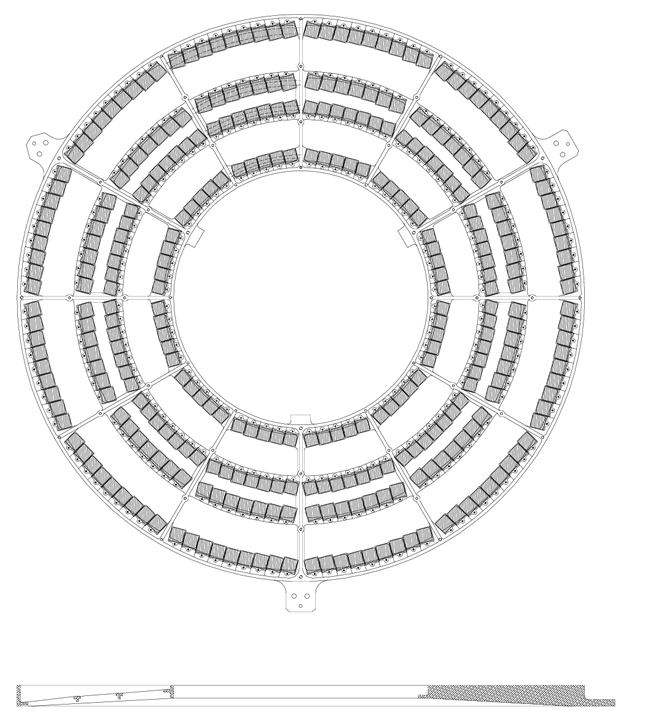
\includegraphics[scale = 0.2]{hess.png}
                \caption{The front and the side view of the HETG structure and the grating facets \citep{ChandraMSFC}.}
                \label{hess}               
                \end{figure}
          \column{0.4\linewidth}
          \begin{itemize}
              \item 192 HEG gratings on the two outer annuli
              \item 144 MEG gratings on the two inner annuli
          \end{itemize}
          \end{columns} 
\end{frame}

\begin{frame}{"X" pattern of the spectra}
    \begin{figure}
        \centering
        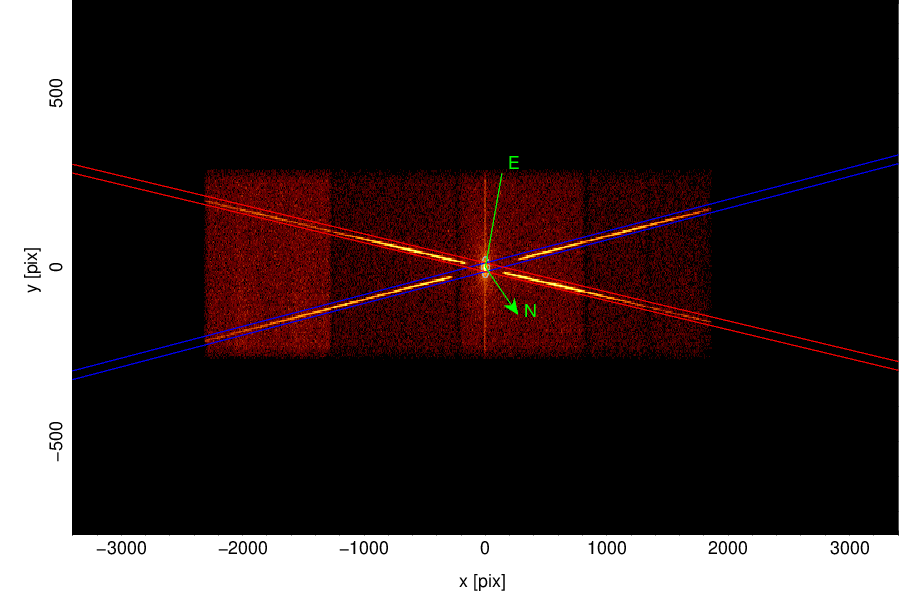
\includegraphics[scale = 0.33]{detailed_X.png}
        \label{xpattern}
    \end{figure}
\end{frame}

\subsection{Strategy}

\begin{frame}{Observation Strategy}
    \begin{figure}
    \centering
    \includemedia[scale = 0.025\linewidth, activate=pageopen, passcontext, transparent, addresource=ss433binary.mp4, flashvars={source=ss433binary.mp4}]{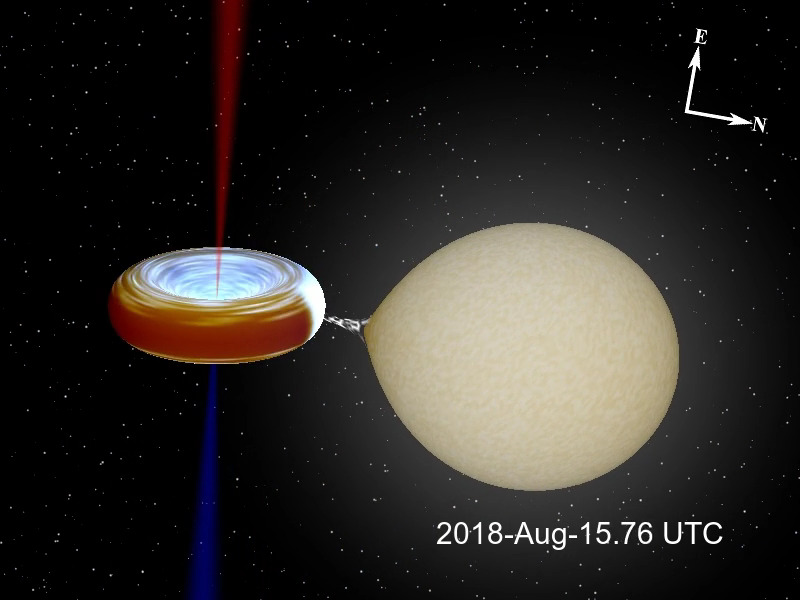
\includegraphics[width=0.07\linewidth]{binary1.jpg}}{VPlayer9.swf}
    %\movie{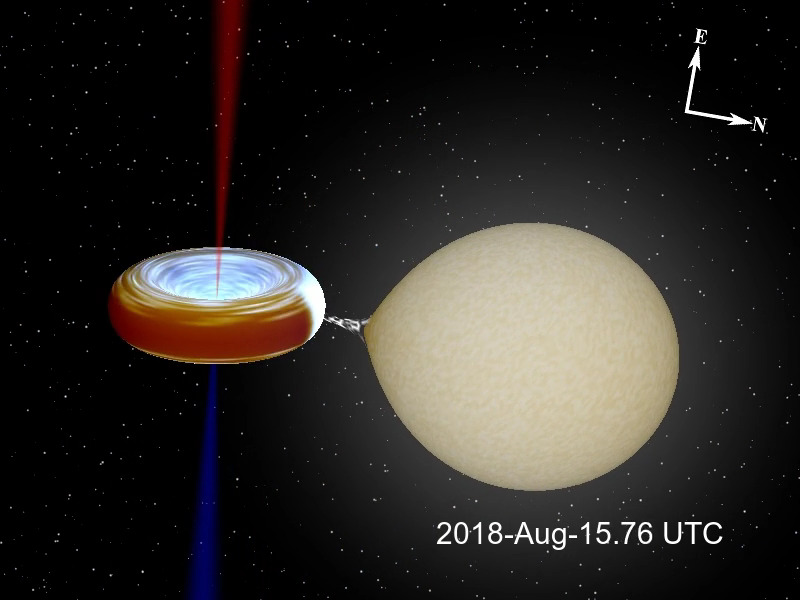
\includegraphics[scale = 0.17]{binary1.jpg}}{ss433_chandra_mjd.mp4}
    \caption{The orbital motion of \href{http://dmaitra.webspace.wheatoncollege.edu/ss433_chandra_mjd.mp4}{ss 433 during our observation}}
    \label{binary}
    \begin{itemize}
        \item A short observation (20 ksec) 3 days before an eclipse.
        \item A long observation (100 ksec, split into 5 parts) starting in the middle of an eclipse.
    \end{itemize}
\end{figure}
    
\end{frame}

\begin{frame}{Spectra Overview}

\begin{figure}
    \centering
    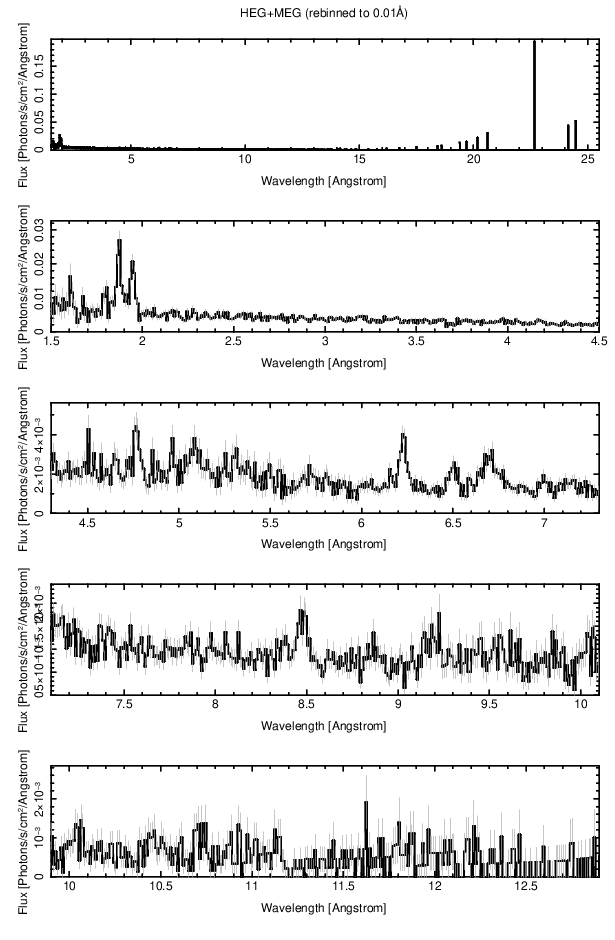
\includegraphics[scale = 0.2]{summaryplot_el.png}
    \caption{Summary plot from TGCAT}
    \label{summary}
\end{figure}
    
\end{frame}

% \begin{frame}{The Periodic Redshifts of Two Jets}
%      \begin{figure}
%         \centering
%         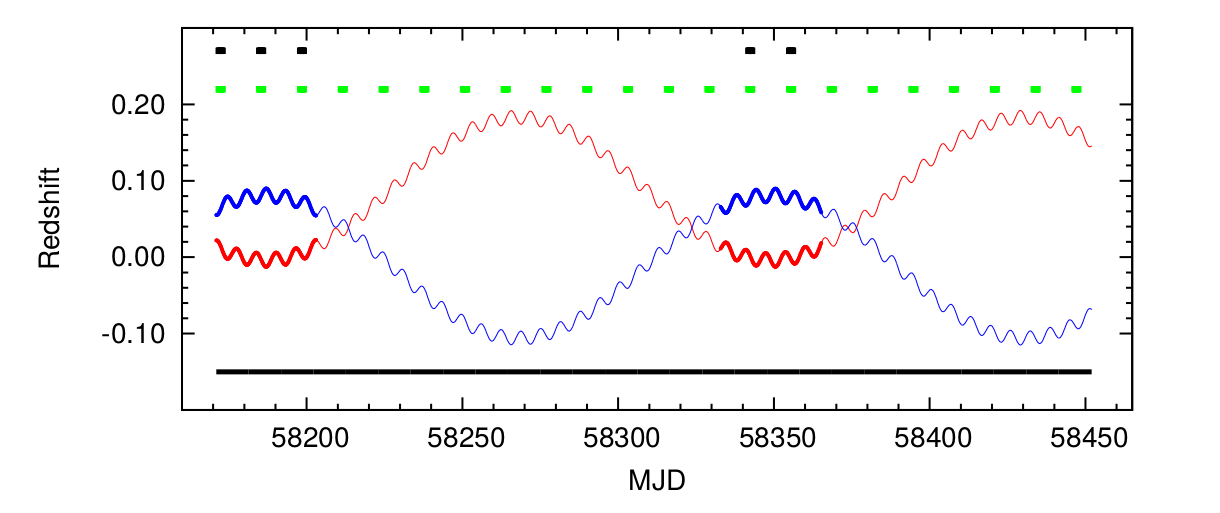
\includegraphics[scale = 0.25]{redshifts_constraint.png}
%         \caption{The red and blue lines indicate the predicted redshifts of the western (which is receding from us most of the time) and the eastern (mostly approaching) jets, including jet-precession and nutation. \citep{Proposal2018}.}
%         \label{redshiftsconstraint}
%     \end{figure}
% \end{frame}

   
    
\section{Investigate two jets with the X-ray spectrum}
\normalsize
\subsection{Spectral Analysis}
\begin{frame}{Fitting Methods}
    \begin{itemize}
        \item Phenomenological fitting models
        \begin{itemize}
            \item Line-grouped fitting method
            \item Blind fitting method
        \end{itemize}
        \item Plasma model
    \end{itemize}
    
\end{frame}


\begin{frame}{Phenomenological fitting}
    \begin{block}{Line-grouped Model \citep{Marshall2002}}
    \begin{itemize}
        \item \textbf{Absorbed Power Law}\par
          $N(E) = KE^{-\alpha}$, where $K$ is photons/keV/cm$^2$/s at 1 keV and $\alpha$ is the photon index. 
         \item \textbf{Gaussian Distributions}\par
          $N(E) = K\dfrac{1}{\sigma \sqrt{2\pi}}exp(\dfrac{-(E-E_l)^2}{2\sigma^2})$ where $K$ is the total photons/cm$^{-2}$/s in the line, $E_l$ is line energy in keV and $\sigma$ is line width in keV.
    \end{itemize}
    \end{block}
\end{frame}

\begin{frame}{Phenomenological fitting in Interative Spectral Interpretation Sys-
tem}
    \begin{block}{Procedures}
    \begin{itemize}
         \item Predict the redshift value based on a kinematic model.
         \item Group emission lines from each jet with Gaussian components of known rest wavelength values.
         \item Derive the best-fitted redshift for each jet based on Cash statistic.
    \end{itemize}
    \end{block}
\end{frame}

\begin{frame}{The Phenomenological Fitting Results}
\begin{figure}
    \centering
    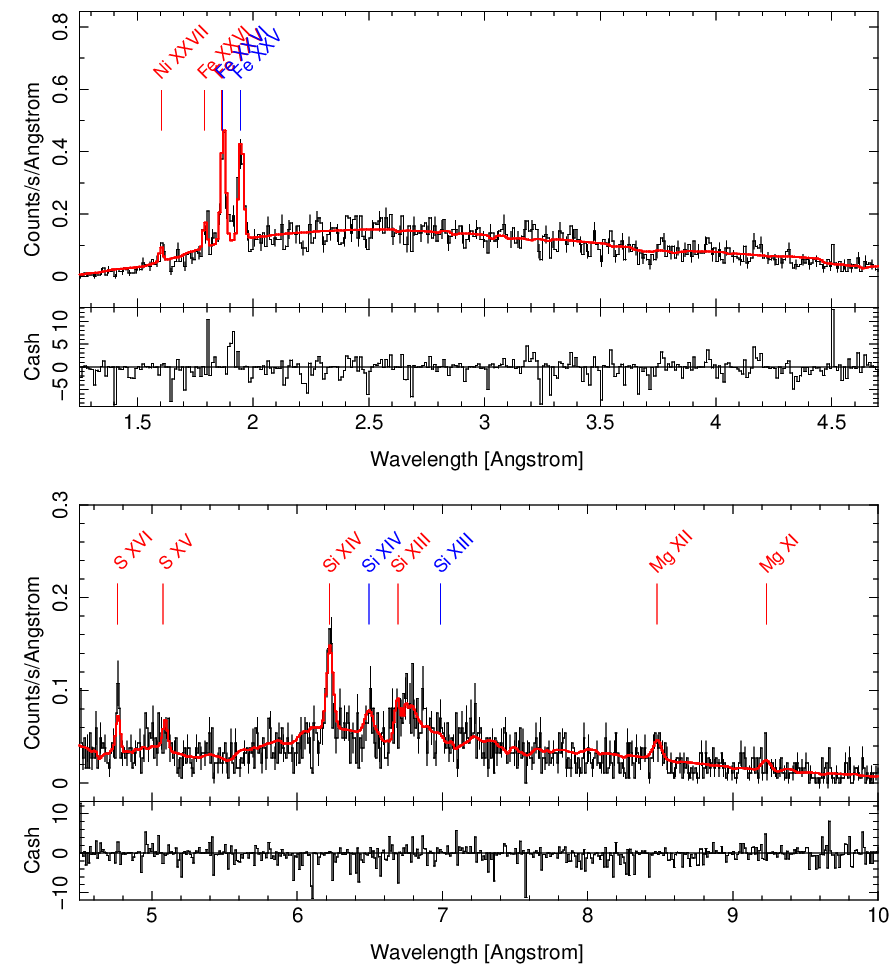
\includegraphics[scale = 0.18]{pheno_short_heg.png}
    \caption{The phenomenological fitting for the HEG spectrum of the short observation. }
    \label{fig:my_label}
\end{figure}
    
\end{frame}

\begin{frame}{The Phenomenological Fitting}
      \begin{columns}
          \column{0.5\linewidth}
            \begin{figure}
                \centering
                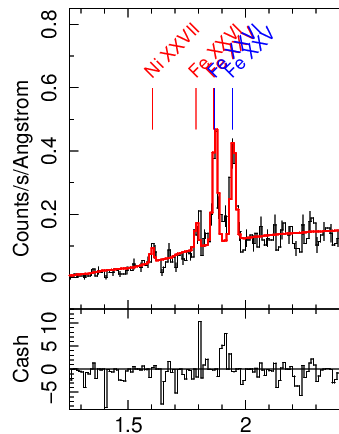
\includegraphics[scale  = 0.39]{short_pheno_part.png}
                \label{plasmashort}               
                \end{figure}
          \column{0.5\linewidth}
            \begin{figure}
                \centering
                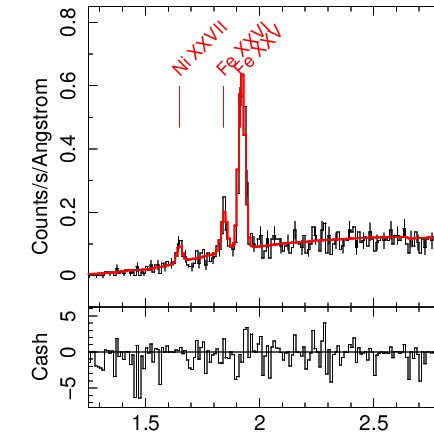
\includegraphics[scale  = 0.37]{long0_part.png}
                \label{plasmashort}               
                \end{figure}
          \end{columns} 

% \begin{tikzpicture}
%   \node (img1) {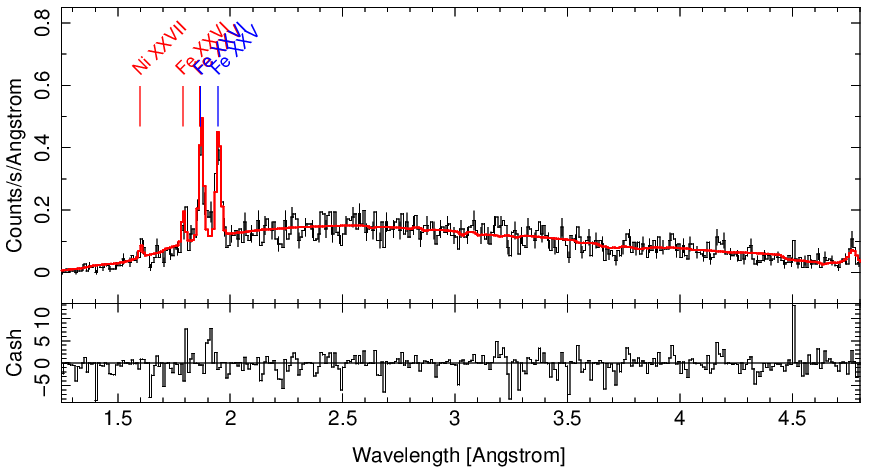
\includegraphics[height=4.2cm]{fittingsh.png}};
%   \pause
%   \node (img2) at (img1.south east)[yshift=1.5cm][xshift=-1cm] {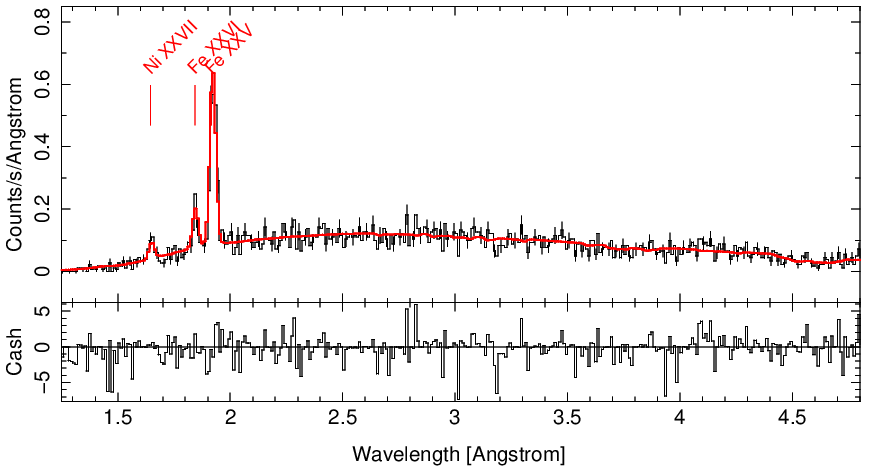
\includegraphics[height=4.2cm] {fitting0.png}};
%   \pause
%   \node (img3) at (img1.south east)[yshift=1.5cm][xshift=-1cm] {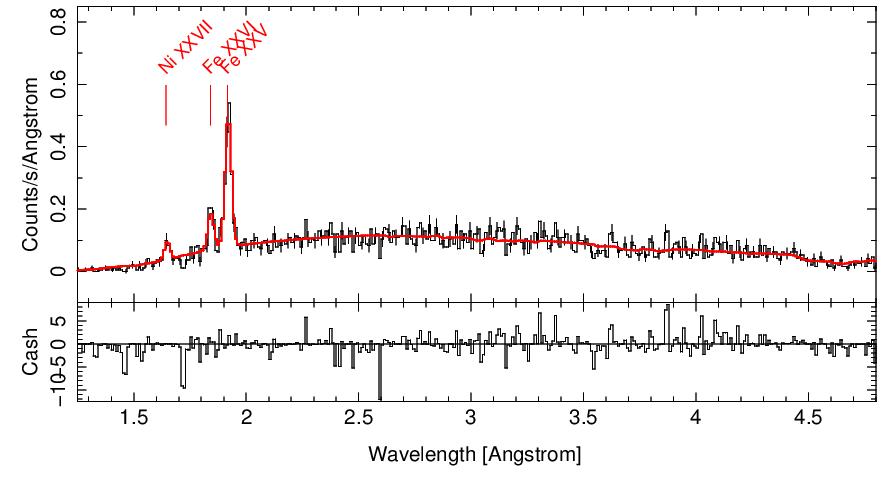
\includegraphics[height=4.2cm] {fitting1.png}};
%   \pause
%   \node (img4) at (img1.south east)[yshift=1.5cm][xshift=-1cm] {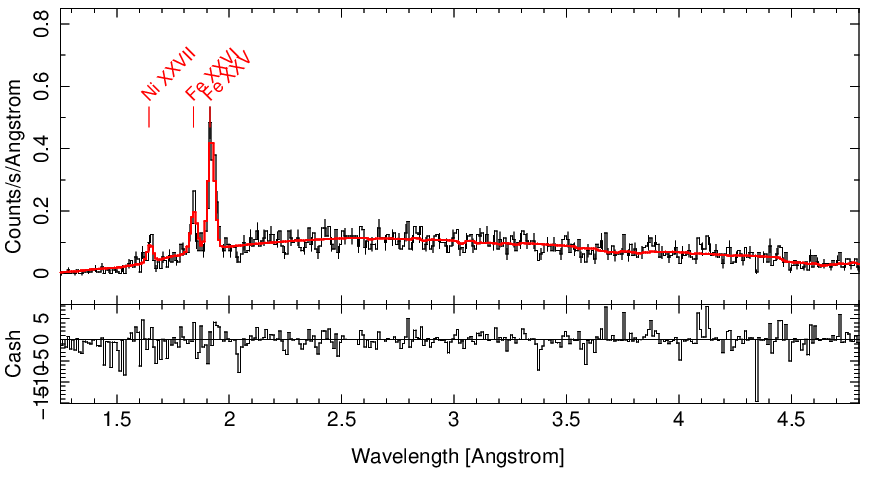
\includegraphics[height=4.2cm] {fitting2.png}};
%   \pause
%   \node (img5) at (img1.south east)[yshift=1.5cm][xshift=-1cm] {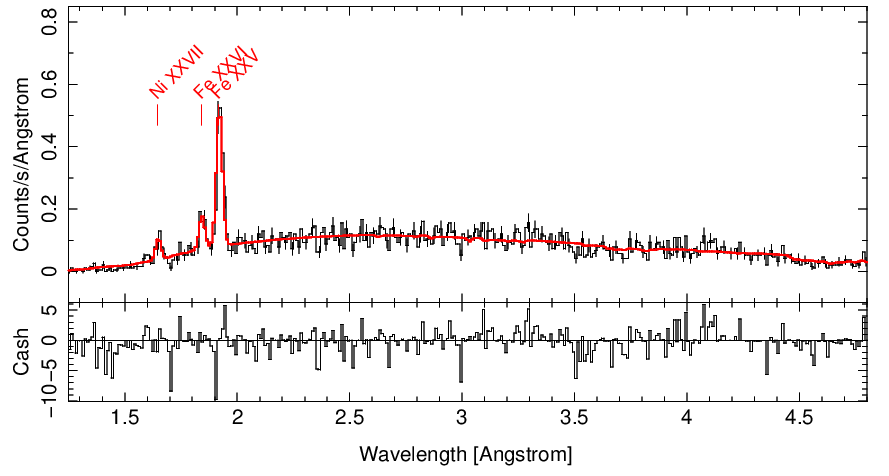
\includegraphics[height=4.2cm] {fitting3.png}};
%   \pause
%   \node (img6) at (img1.south east)[yshift=1.5cm][xshift=-1cm] {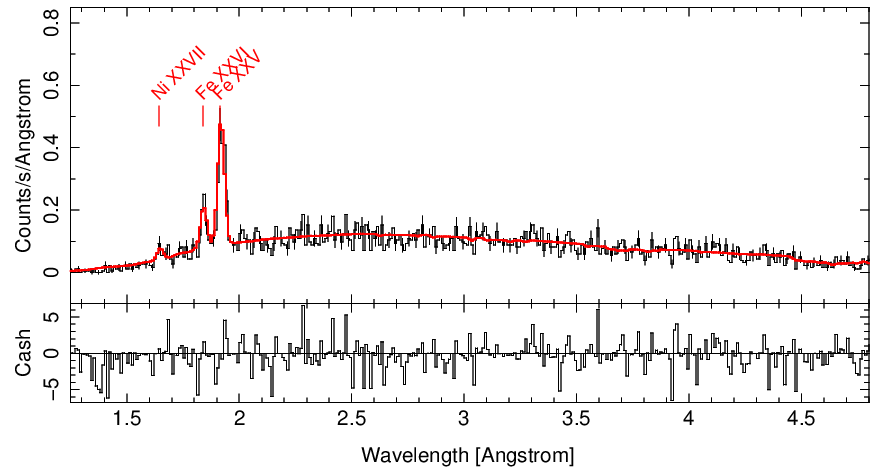
\includegraphics[height=4.2cm] {fitting4.png}};
  
% \end{tikzpicture}
% \captionof{figure}{The phenomenological fitting for the spectrum of the short and long observation.}

\end{frame}


%-----------------------------------------------------
%----------------------------------------------------
%----------------Blind Fitting------------------------
\begin{frame}{The Phenomenological Fitting Results}
Redshifts for the Western jet in the short observation
\begin{itemize}
    \item Predicted: -0.0097 $\pm$ 0.009
    \item Observed: 0.034 $\pm$ 0.0002
\end{itemize}

\begin{block}{Blind Fitting Method \citep{Marshall2002}}
Differences from the line-grouped method:
    \begin{itemize}
         \item Fit the emission lines using Voigt profiles.
         \item The line fitting is independent of redshift.
         \item Being able to distinguish the Fe {\sc xv} from the Western jet and Fe {\sc xxvi} from the Eastern jet.
    \end{itemize}
\end{block}
    
\end{frame}


\begin{frame}{SS 433 Redshifts of the Western Jet Lines Using Voigt Profile}
\begin{figure}
    \centering
    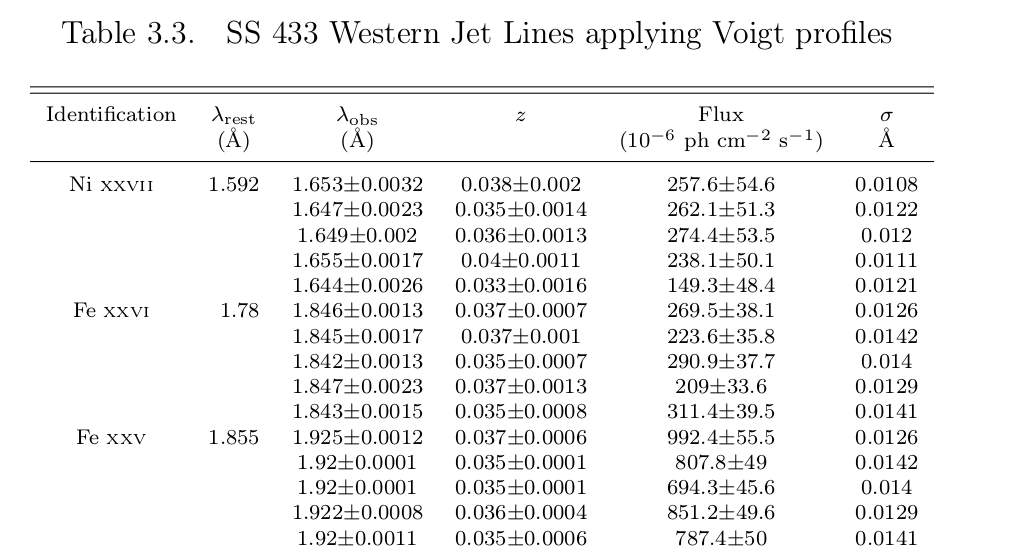
\includegraphics[scale = 0.28]{linetable.png}
    \label{westlongz}
\end{figure}


    
\end{frame}
%-------------------------------------------------
%--------------------------------------------

\begin{frame}{Plasma Model}
    \begin{block}{Plasma}
    Plasma is an electrically neutral medium that consists of a mixture of electrons and ions.
    \end{block}
    \begin{block}{Plasma Model}
    \textbf{Four-temperature} plasma model with parameters of temperatures, metal abundance, redshift, turbulent velocity and normalization (emission measure) \citep{Marshall2002}.
    \end{block}
\end{frame}

\begin{frame}{Plasma Model Fitting to the Short Observation}
      \begin{columns}
          \column{0.25\linewidth}
            \begin{figure}
                \centering
                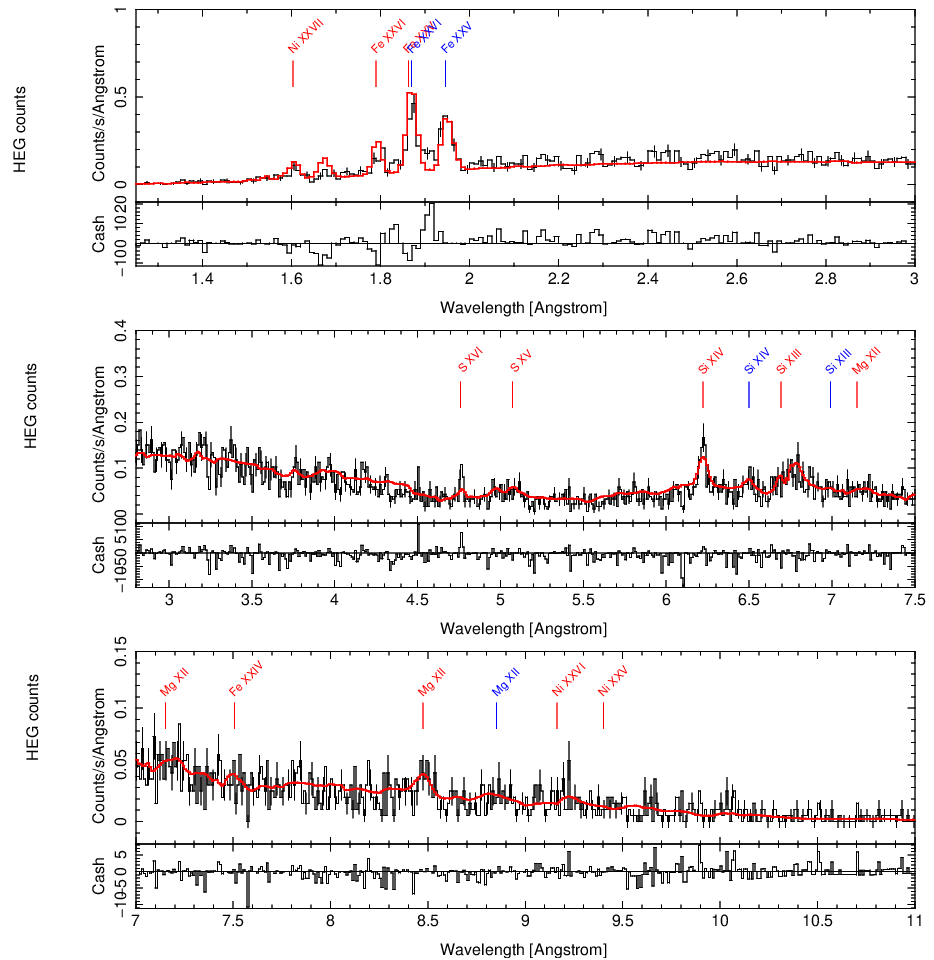
\includegraphics[scale  = 0.2]{plasmashort_heg.png}
                \label{plasmashort}       
                \end{figure}
    \pause
          \column{0.7\linewidth}
            \begin{figure}
                \centering
                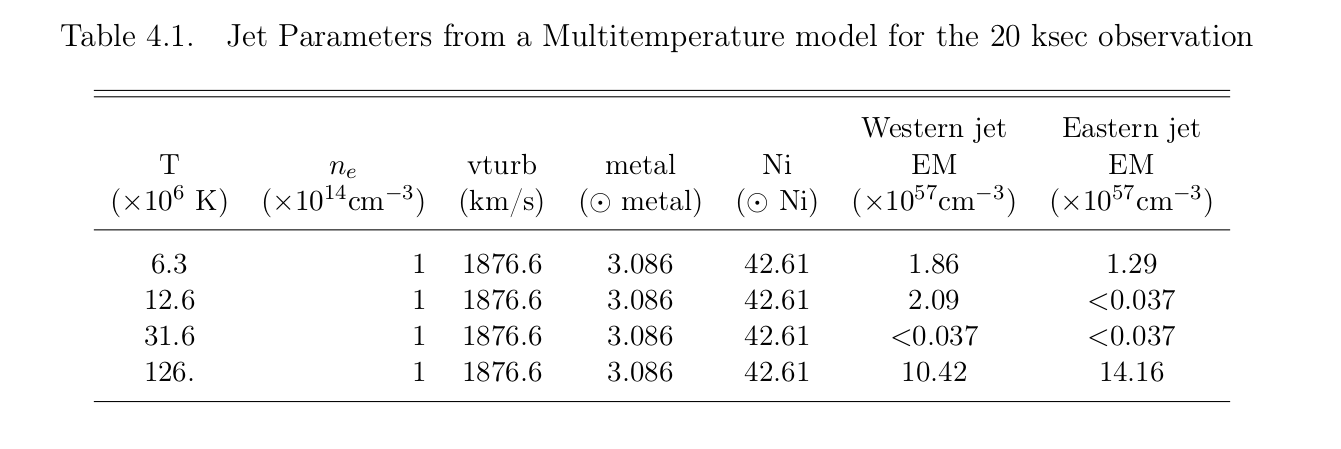
\includegraphics[scale  = 0.17]{plasma_short_table.png}
                \label{plasmashort}               
                \end{figure}
          \end{columns} 
    % \begin{figure}
    %     \centering
    %     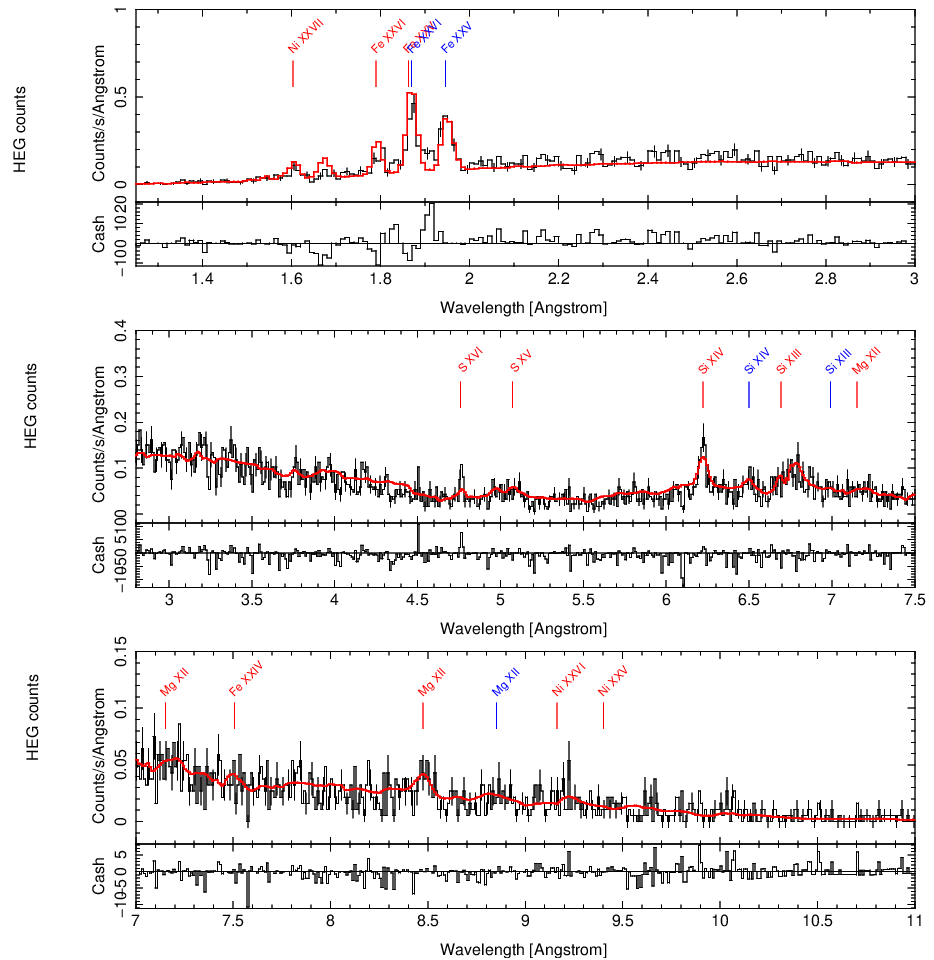
\includegraphics[scale  = 0.22]{plasmashort_heg.png}
    %     \label{plasmashort}
    % \end{figure}
    % \begin{figure}
    %     \centering
    %     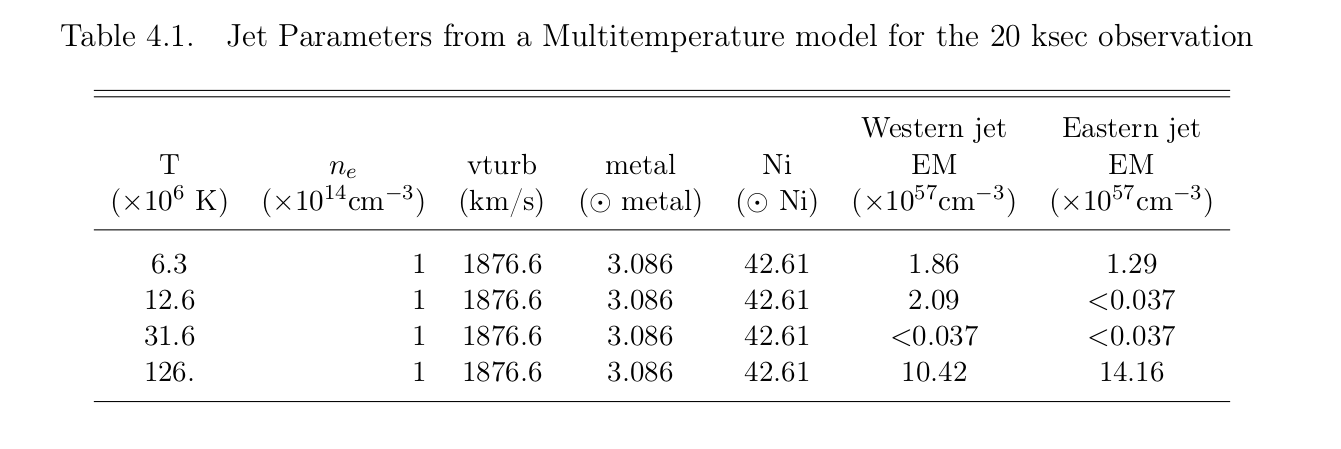
\includegraphics[scale  = 0.13]{plasma_short_table.png}
    %     \label{plasmatable}
    % \end{figure}
        

\end{frame}

%------------------------------------------
%-------------------------------------
\section{Discussions and Conclusions}

\subsection{Redshift Discrepancy}
\begin{frame}{The Redshift Variations over the Short and Long Observations}
    \begin{figure}
        \centering
        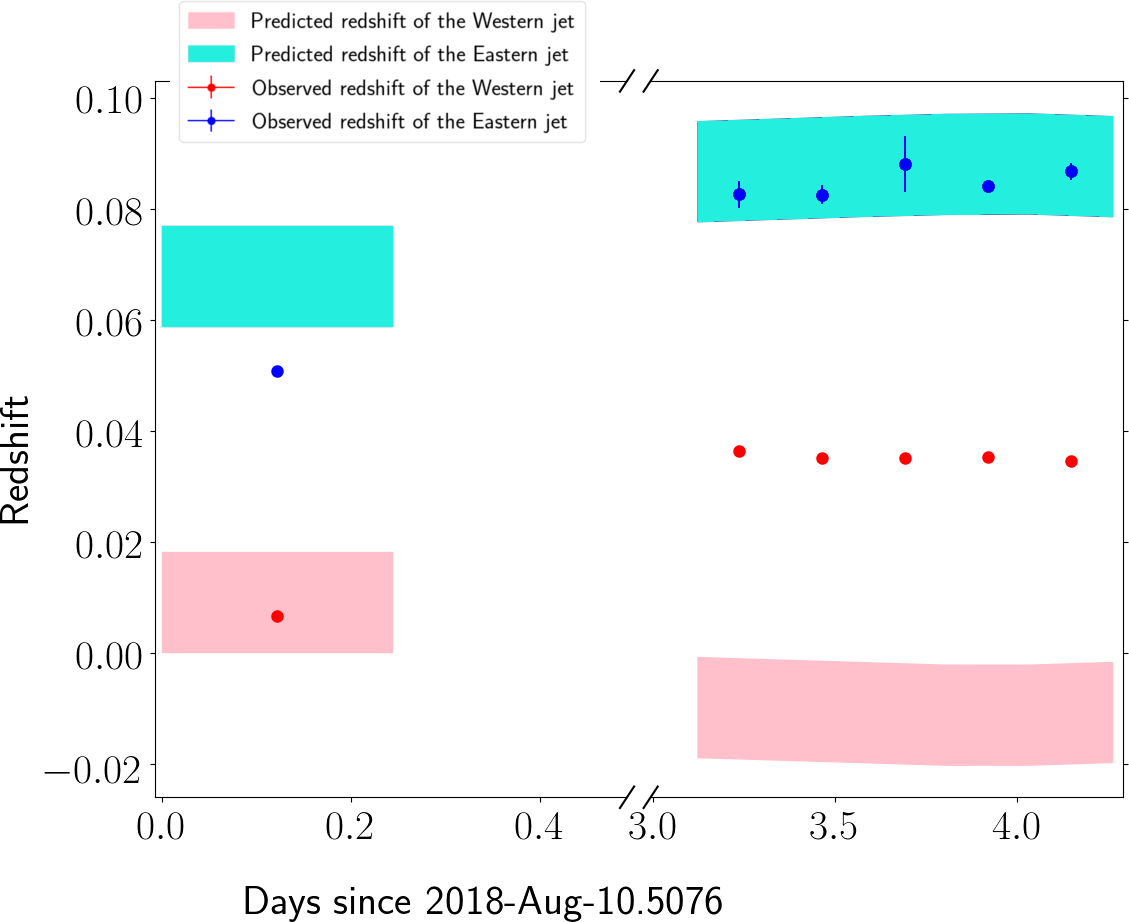
\includegraphics[scale = 0.22]{redshiftv7.png}
        \label{redshiftschange}
    \end{figure}
\end{frame}


\begin{frame}{Velocity of the jet $v$ and angle between line of sight and the jet $\theta$}

\begin{figure}
    \centering
    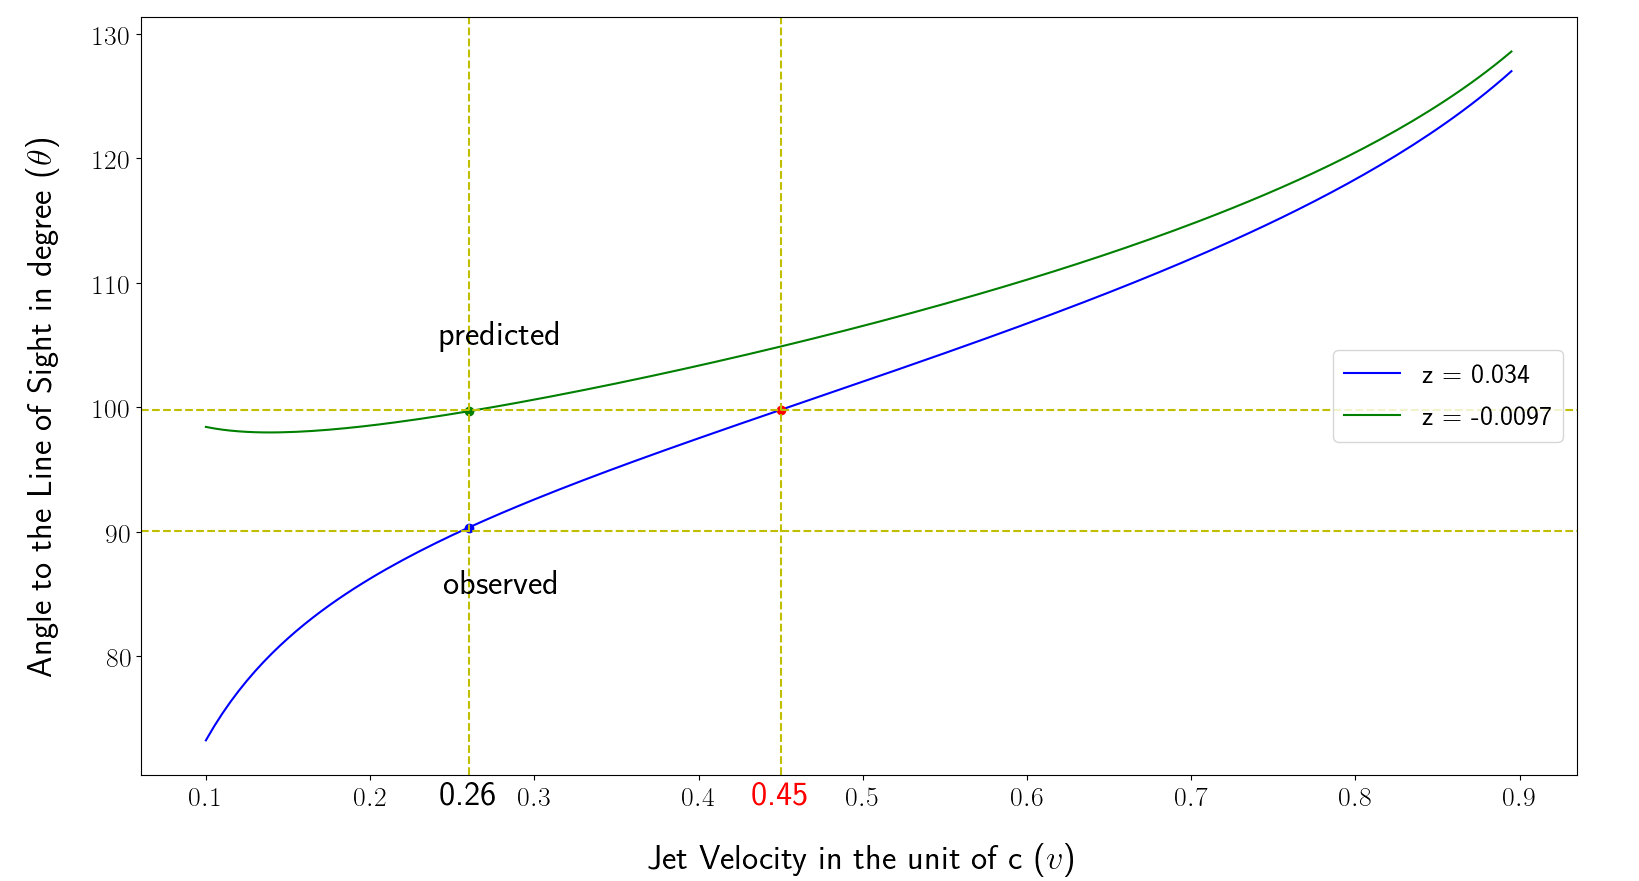
\includegraphics[scale = 0.17]{thetav2.png}
    \label{thetav}
\end{figure}
    
\end{frame}
%------------------------------------------

\begin{frame}{The Line flux Variations of the Western Jet}
    \begin{figure}
        \begin{figure}
            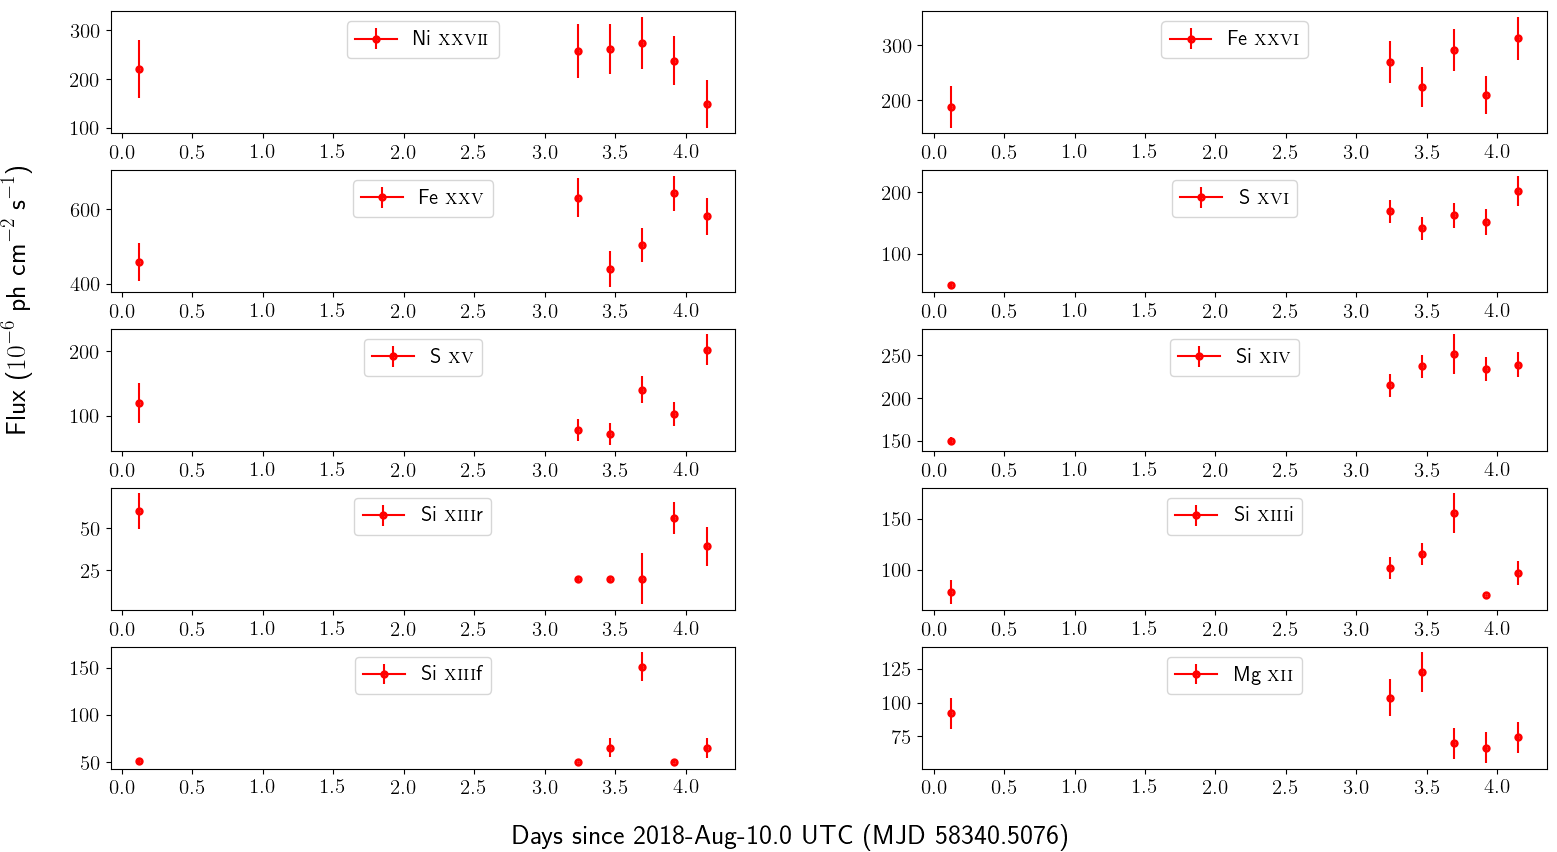
\includegraphics[scale = 0.17]{west_flux.png}
            \label{west_flux}
        \end{figure}
    \end{figure}
\end{frame}


\subsection{Line Flux Change}
\begin{frame}{The Line flux Variations of the Eastern Jet}
\begin{figure}
    \centering
    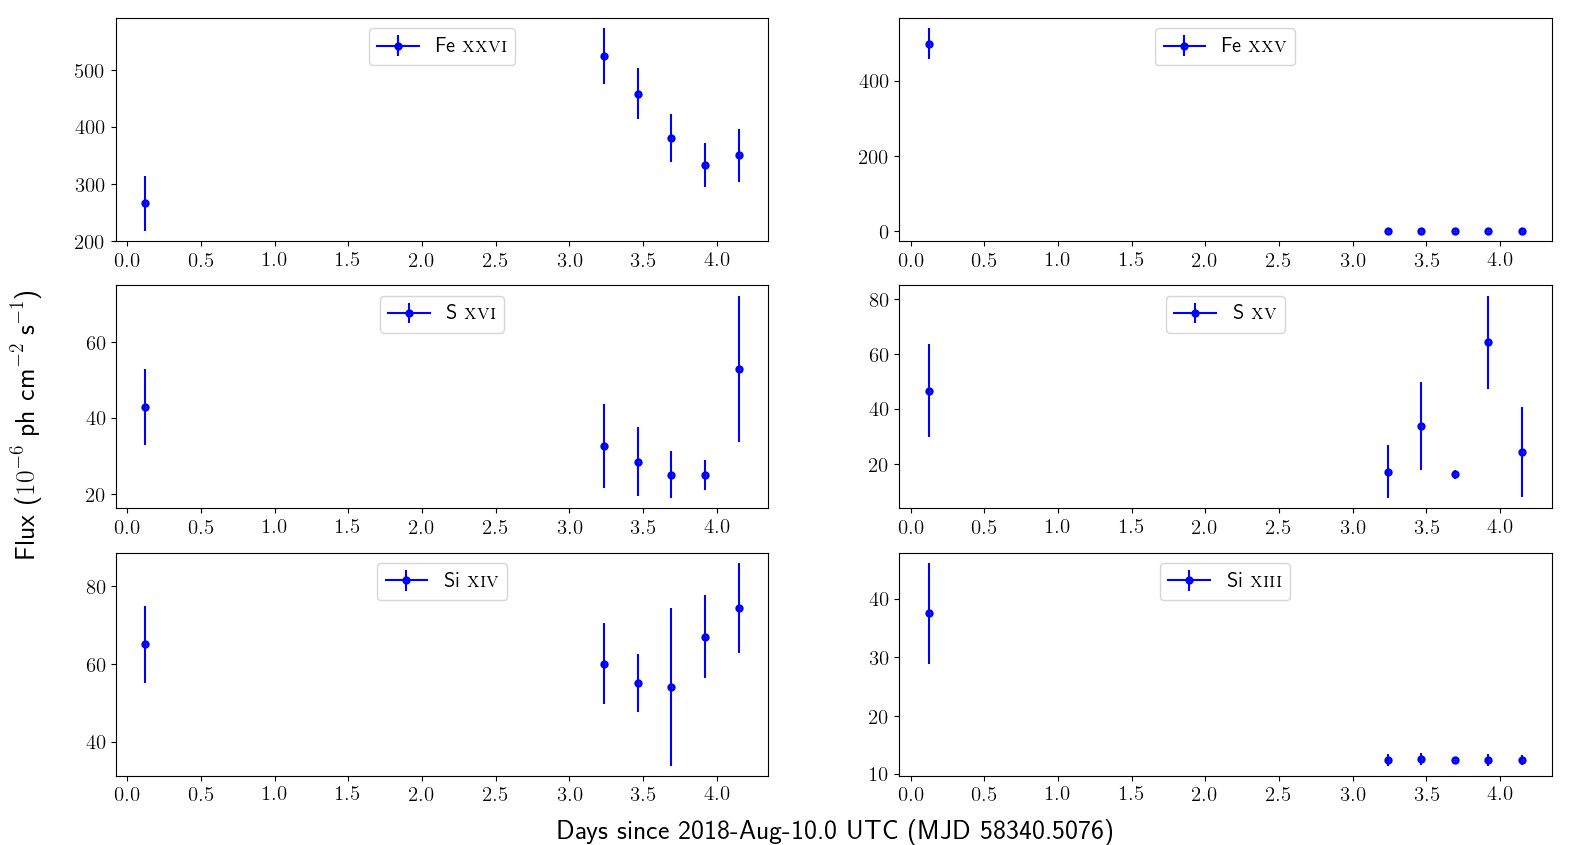
\includegraphics[scale = 0.17]{east_flux.png}
    \label{east_flux}
\end{figure}
%     \begin{tikzpicture}[remember picture,overlay]
%         \node[xshift =5cm, yshift = 3.8cm] at (current page.south west) {
%         \parbox{0.87\textwidth}{
%         \begin{figure}
%             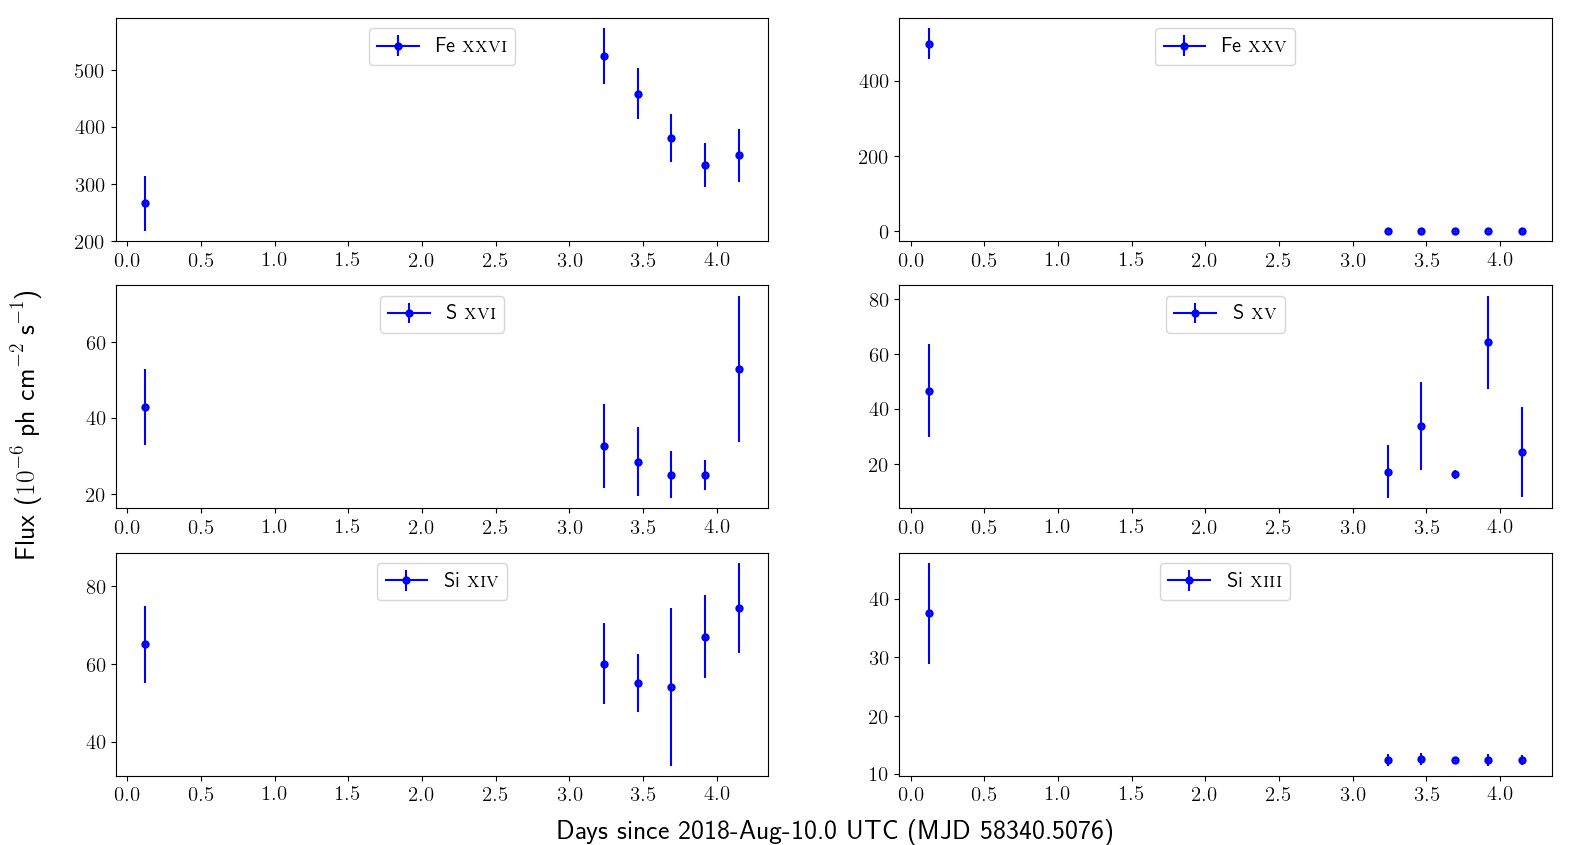
\includegraphics[scale = 0.2]{east_flux.png}
%             \label{east_flux}
%         \end{figure}
%         }};
%     \end{tikzpicture}
% \pause
%     \begin{tikzpicture}[remember picture, overlay]
%         \node[xshift=-2cm,yshift=-3cm] at (current page.north east) {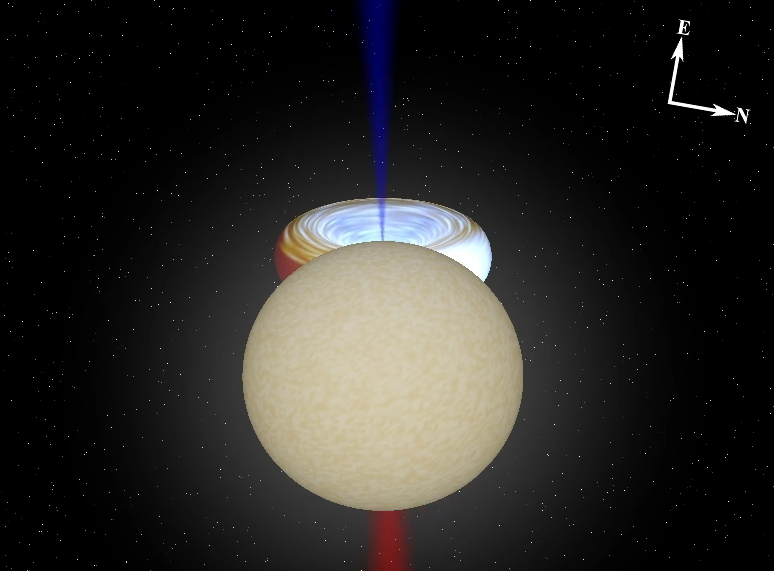
\includegraphics[scale = 0.1]{jet.png}};
%     \end{tikzpicture}
\end{frame}




\subsection{Continuum Spectrum}

\begin{frame}{Power Law}
        \begin{figure}
            \centering
            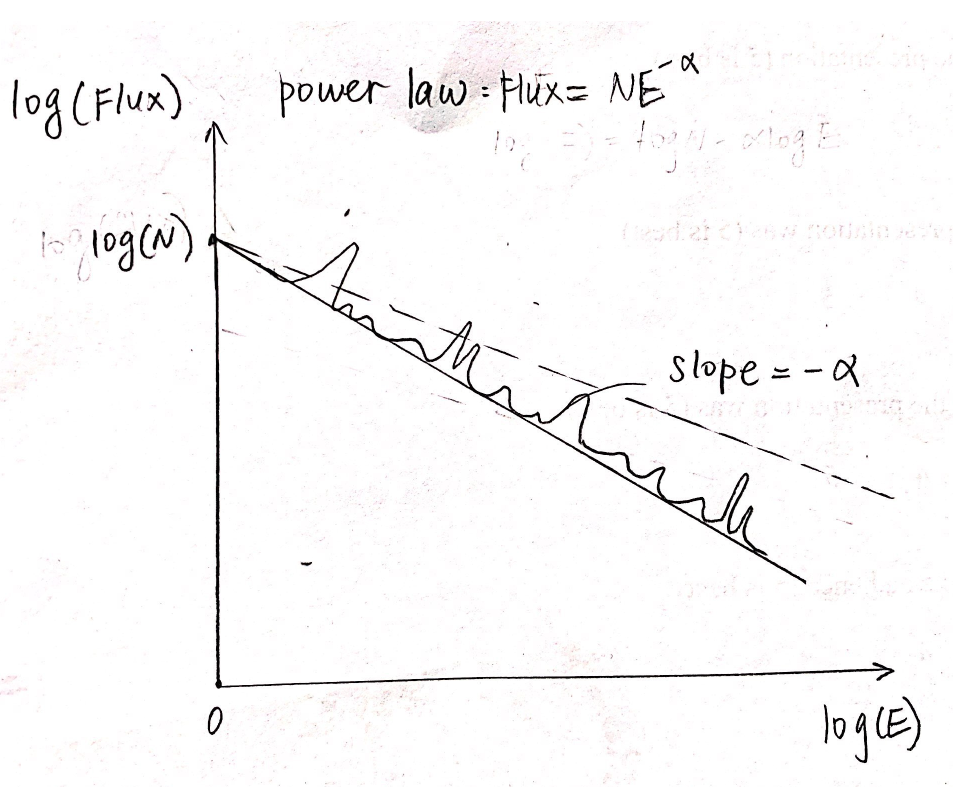
\includegraphics[scale = 0.2]{powerlaw_v2.png}
            \label{pl}
        \end{figure}
\end{frame}

\begin{frame}{Normalization of the Power Law}
            \begin{figure}
                \centering
                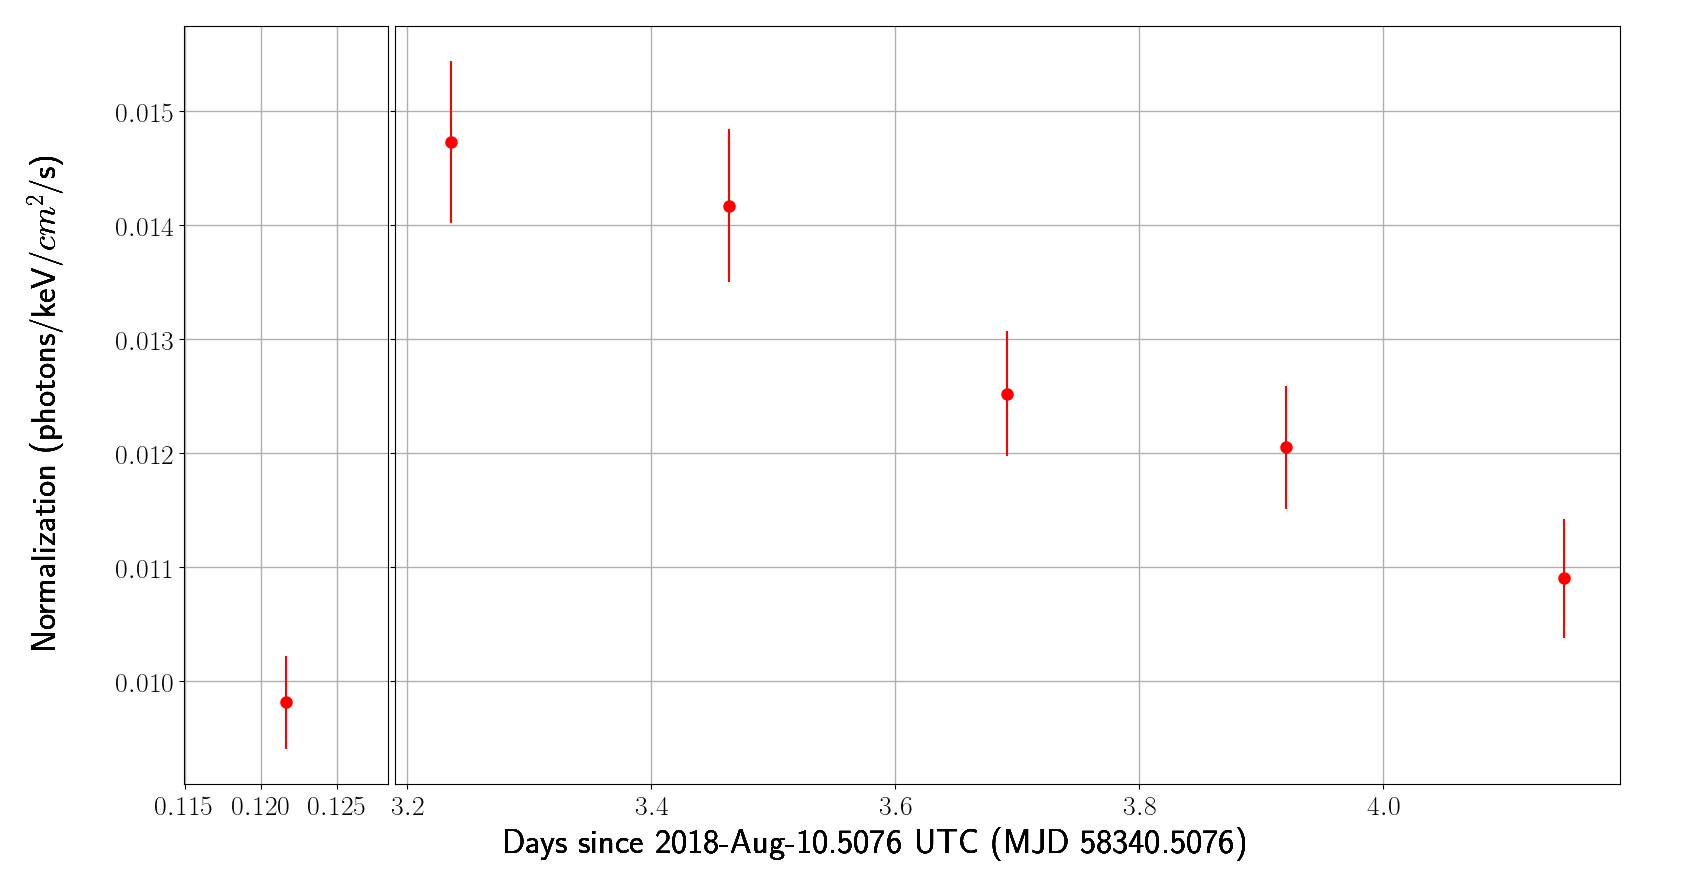
\includegraphics[scale = 0.18]{pl_norm.png}
                \label{norm_pl}
            \end{figure}
\end{frame}

\begin{frame}{Photon Index of the Power Law}
            \begin{figure}
                \centering
                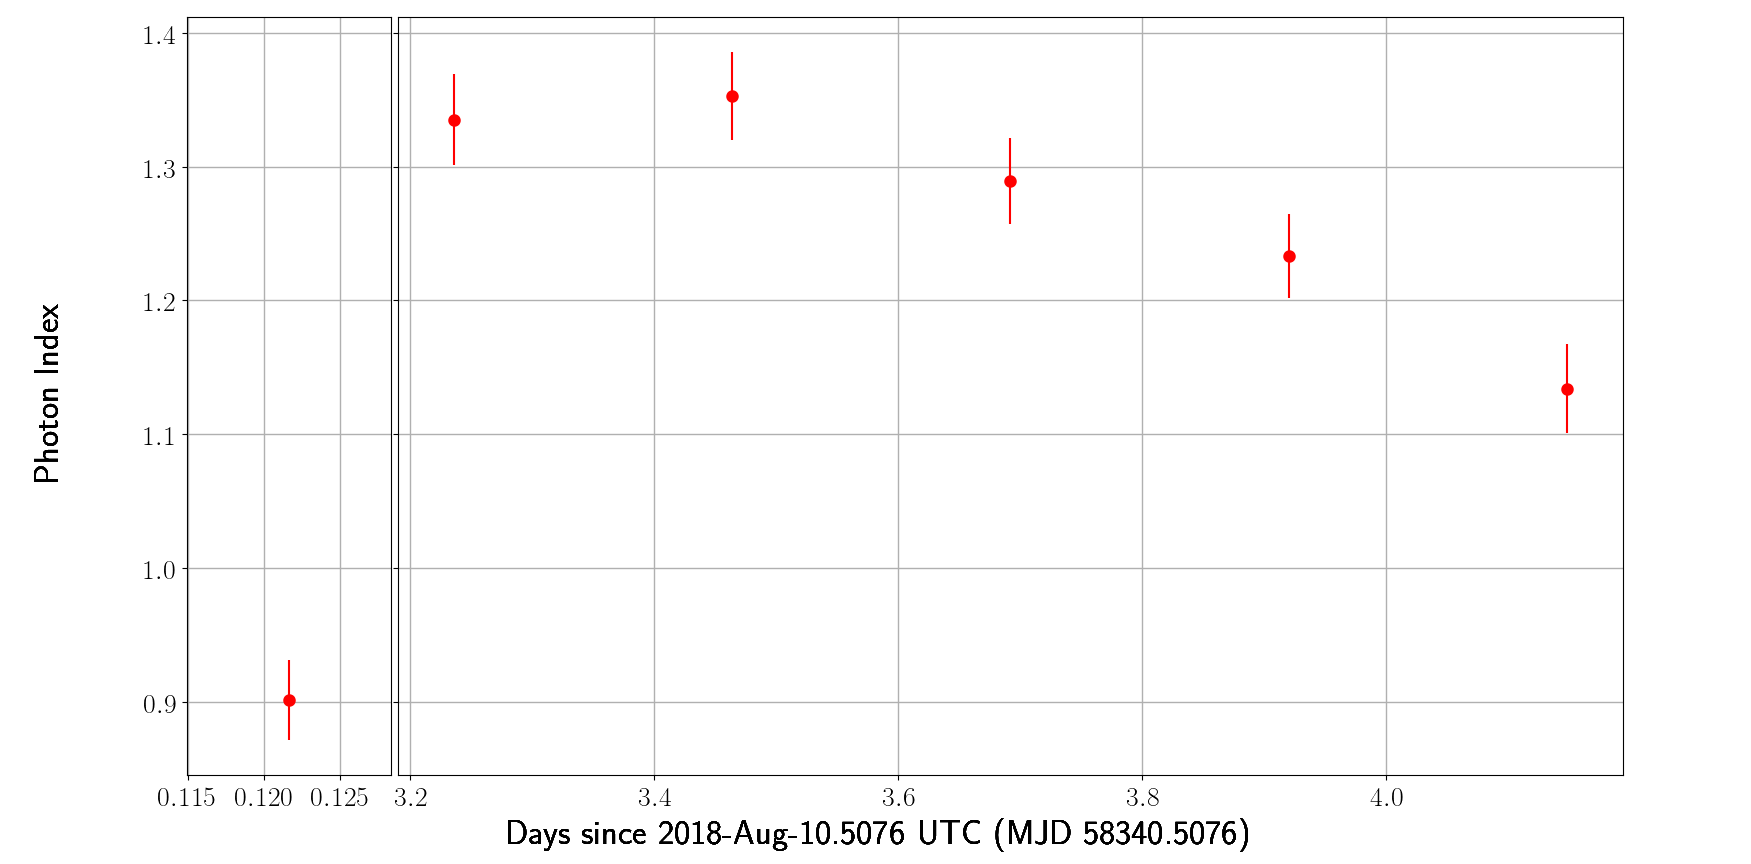
\includegraphics[scale = 0.17]{pl_photon.png}
                \label{photon_pl}
            \end{figure}
\end{frame}






\subsection{}
\normalsize
\begin{frame}{Conclusion}
\begin{itemize}
    \item The Western and Eastern jets move independently at the X-rays.
    \item The Western jet was likely not affected by the eclipse.
    \item The portion of the Eastern jet being blocked is uncertain.
    \item Contrary to our expectations, the intrinsic accretion flow might be changing during our observation.
\end{itemize}
\end{frame}


\begin{frame}{References}
    \bibliography{reference}
\end{frame}

\begin{frame}{Acknowledgements}
\textbf{Many thanks to} 


\end{frame}




% \begin{frame}{Why is SS 433 so Special?}
%     \begin{itemize}
%         \item The first discovered radio-jet \href{ http://dmaitra.webspace.wheatoncollege.edu/ss433_chandra_mjd.mp4}{X-ray binary system} 5.5 kpc away from us.\par
%         \item A pair of oppositely directed jets with a velocity of 0.26c.
%         \item The only source that is known to have emission lines from ionized gas in the jet from the compact object.
%         \item (The orbit period is about 13.1 days. The jet precesses with a 162.5 day period in a cone with half-angle 19\textdegree.85 about an axis that is 78\textdegree.83 to the line of sight.)
%     \end{itemize}
    
% \end{frame}


\begin{frame}{Chandra Overview}
       \begin{columns}
          \column{0.45\linewidth}
            \begin{figure}
                \centering
                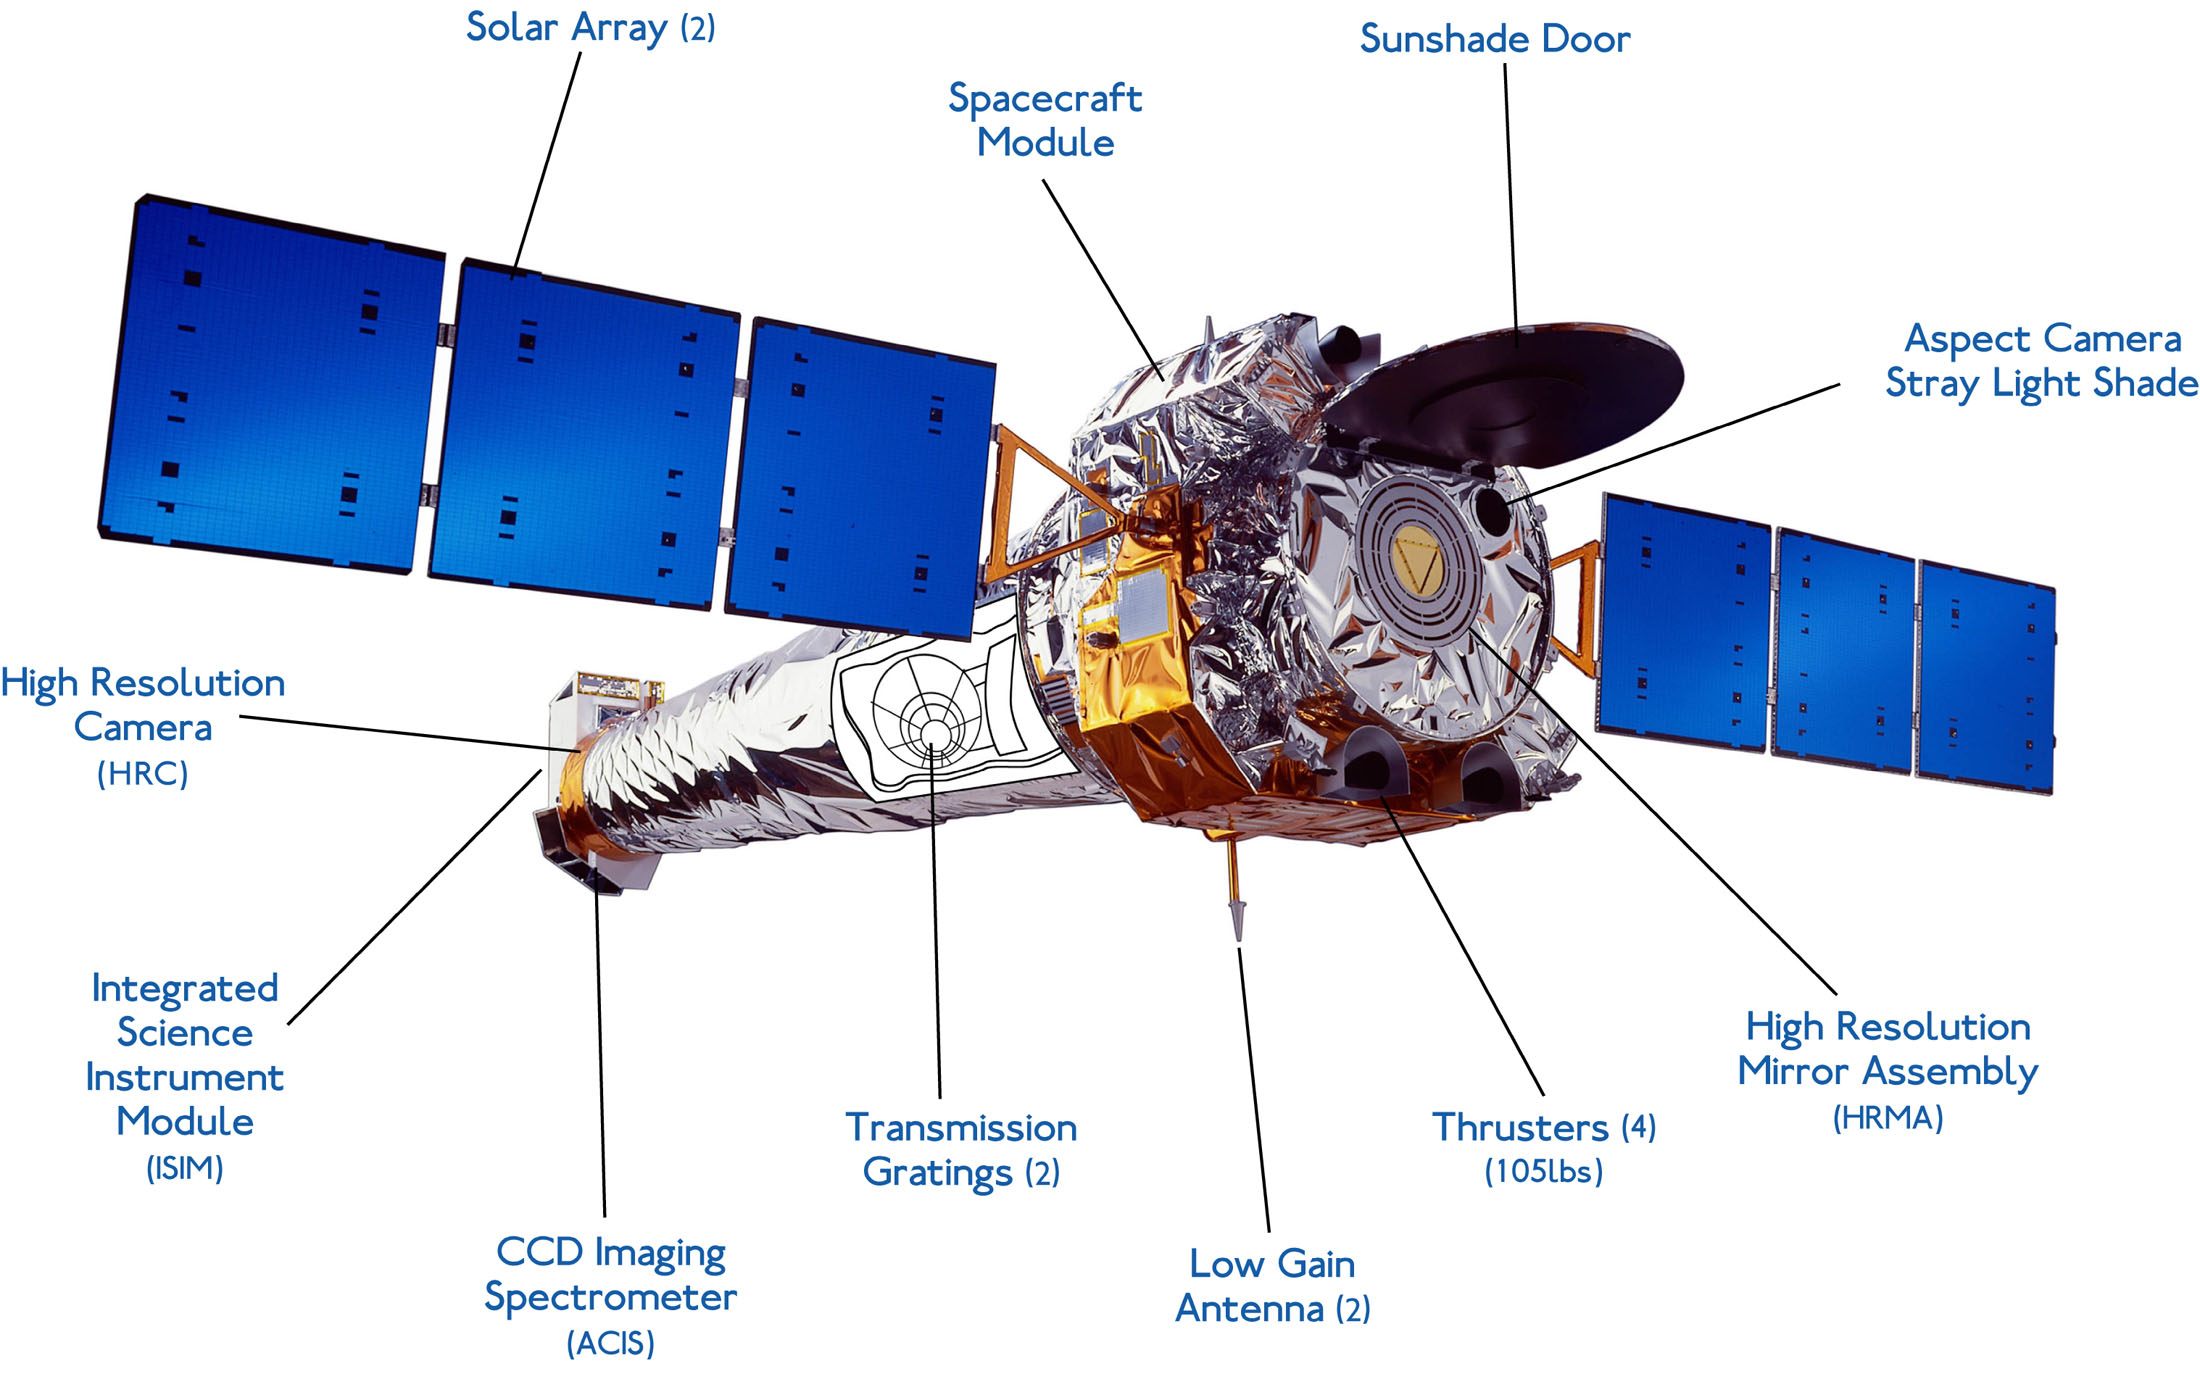
\includegraphics[scale = 0.3]{chandra_full.jpg}
                \caption{The Chandra Telescope with main components labeled \citep{Harbaugh2017}.}
                \label{Chandratelescope}               \end{figure}
          \column{0.4\linewidth}
          \begin{itemize}
              \item High Resolution Mirror Assembly (HRMA)
              \item Advanced CCD Imaging Spectrometer (ACIS)
              \item High Resolution Camera (HRC)
              \item \textbf{High Energy Transmission Grating (HETG)} and Low Energy Transmission Grating (LETG) together covered the energy range from ($\leq$ 0.1 to 10 keV)
          \end{itemize}
          \end{columns} 
\end{frame}


\begin{frame}{Kinematic Model}
$(1+z) = \gamma (\pm vsin\theta sin i cos\phi \pm vcos\theta cos i) +1$
where $\theta$ is the jet precession angle, $i$ is the angle between the jet axis to our line of sight, $\phi = \phi_0 + 2\pi (t-t_0)/P_0$, where $P_0$ is the date of (Feb 22, 1978).
    
\end{frame}



\begin{frame}{Voigt Profile}
Voigt profile is the convolution
of the natural resonance of an emitted line with the Maxwellian speed distribution. The natural resonance profile is a Lorentzian with full-width at half
maximum. The natural resonance profile is a Lorentzian with full-width at half
maximum. The Maxwellian speed distribution is a Gaussian with velocity width $v_0 = (\dfrac{2kT}{m})^{1/2}$, where $m$ is the ion mass and $T$ is the temperature.
    
\end{frame}

\begin{frame}{Emission Measure}
The observed flux of an emission line from a region of plasma with electron density $n_e$ and temperature $T$ is given by

\begin{equation*}
    f_i = \dfrac{J_i(T)\int n_en_H dV }{4\pi D^2} = \dfrac{J_i(T)EM(T)}{4\pi D^2}
\end{equation*}
where D is the distance from the Earth to the source, in our case, 5.5 kpc, $n_H$ is the density of the hydrogen and EM is the emission measure.\par 

EM can be found using the definition of normalizations in the default plasma function in ISIS,
\begin{equation*}
    \mathrm{norm} = \dfrac{1\times 10^{-14}}{4\pi D^2}\int n_e n_H dV =  \dfrac{1\times 10^{-14}}{4\pi D^2} EM
\end{equation*}
\end{frame}


\scriptsize
\begin{frame}{Estimate the radius using the geometry}
       \begin{columns}
          \column{0.58\linewidth}
            \begin{figure}
                \centering
                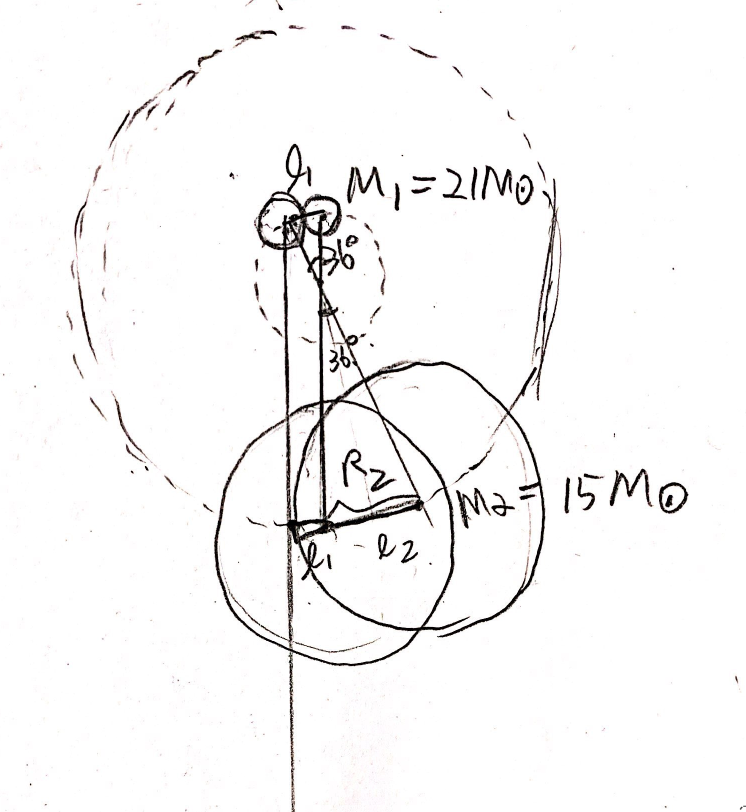
\includegraphics[scale = 0.2]{geometry_radius.jpg}
                \caption{The geometry of the binary system}
                \label{geometry_radius}
            \end{figure}
            
           \column{0.6\linewidth}
            Assume the mass of the compact object is 21 $M_{\odot}$ and the mass of the companion object is 15 $M_{\odot}$ \citep{Bowler2018}. And the binary separation $a$ is $5.3 \times 10^7$ km. \par
            The radius of the orbits are 
            \begin{align*}
                a_1 &= (\dfrac{m_2}{m_1 + m_2})a = 2.2\times10^7 \mathrm{km}\\
                a_2 &= (\dfrac{m_1}{m_1 + m_2})a = 3.1\times10^7 \mathrm{km}
            \end{align*}
            Since the orbital phase of the accretor at the end of our observation was 0.1, then
              \begin{align*}
                L1 &= 0.2\pi(2.2\times10^7) km\\
                L2 &= 0.2\pi(3.1\times10^7) km\\
                R &\sim L1 + L2 = 47.9 R_{\odot}
             \end{align*}
         \end{columns} 
    
\end{frame}




\end{document}


